% Options for packages loaded elsewhere
\PassOptionsToPackage{unicode}{hyperref}
\PassOptionsToPackage{hyphens}{url}
%
\documentclass[
  english,
  man]{apa6}
\usepackage{amsmath,amssymb}
\usepackage{lmodern}
\usepackage{ifxetex,ifluatex}
\ifnum 0\ifxetex 1\fi\ifluatex 1\fi=0 % if pdftex
  \usepackage[T1]{fontenc}
  \usepackage[utf8]{inputenc}
  \usepackage{textcomp} % provide euro and other symbols
\else % if luatex or xetex
  \usepackage{unicode-math}
  \defaultfontfeatures{Scale=MatchLowercase}
  \defaultfontfeatures[\rmfamily]{Ligatures=TeX,Scale=1}
\fi
% Use upquote if available, for straight quotes in verbatim environments
\IfFileExists{upquote.sty}{\usepackage{upquote}}{}
\IfFileExists{microtype.sty}{% use microtype if available
  \usepackage[]{microtype}
  \UseMicrotypeSet[protrusion]{basicmath} % disable protrusion for tt fonts
}{}
\makeatletter
\@ifundefined{KOMAClassName}{% if non-KOMA class
  \IfFileExists{parskip.sty}{%
    \usepackage{parskip}
  }{% else
    \setlength{\parindent}{0pt}
    \setlength{\parskip}{6pt plus 2pt minus 1pt}}
}{% if KOMA class
  \KOMAoptions{parskip=half}}
\makeatother
\usepackage{xcolor}
\IfFileExists{xurl.sty}{\usepackage{xurl}}{} % add URL line breaks if available
\IfFileExists{bookmark.sty}{\usepackage{bookmark}}{\usepackage{hyperref}}
\hypersetup{
  pdflang={en-EN},
  hidelinks,
  pdfcreator={LaTeX via pandoc}}
\urlstyle{same} % disable monospaced font for URLs
\usepackage{graphicx}
\makeatletter
\def\maxwidth{\ifdim\Gin@nat@width>\linewidth\linewidth\else\Gin@nat@width\fi}
\def\maxheight{\ifdim\Gin@nat@height>\textheight\textheight\else\Gin@nat@height\fi}
\makeatother
% Scale images if necessary, so that they will not overflow the page
% margins by default, and it is still possible to overwrite the defaults
% using explicit options in \includegraphics[width, height, ...]{}
\setkeys{Gin}{width=\maxwidth,height=\maxheight,keepaspectratio}
% Set default figure placement to htbp
\makeatletter
\def\fps@figure{htbp}
\makeatother
\setlength{\emergencystretch}{3em} % prevent overfull lines
\providecommand{\tightlist}{%
  \setlength{\itemsep}{0pt}\setlength{\parskip}{0pt}}
\setcounter{secnumdepth}{-\maxdimen} % remove section numbering
% Make \paragraph and \subparagraph free-standing
\ifx\paragraph\undefined\else
  \let\oldparagraph\paragraph
  \renewcommand{\paragraph}[1]{\oldparagraph{#1}\mbox{}}
\fi
\ifx\subparagraph\undefined\else
  \let\oldsubparagraph\subparagraph
  \renewcommand{\subparagraph}[1]{\oldsubparagraph{#1}\mbox{}}
\fi
% Manuscript styling
\usepackage{upgreek}
\captionsetup{font=singlespacing,justification=justified}

% Table formatting
\usepackage{longtable}
\usepackage{lscape}
% \usepackage[counterclockwise]{rotating}   % Landscape page setup for large tables
\usepackage{multirow}		% Table styling
\usepackage{tabularx}		% Control Column width
\usepackage[flushleft]{threeparttable}	% Allows for three part tables with a specified notes section
\usepackage{threeparttablex}            % Lets threeparttable work with longtable

% Create new environments so endfloat can handle them
% \newenvironment{ltable}
%   {\begin{landscape}\centering\begin{threeparttable}}
%   {\end{threeparttable}\end{landscape}}
\newenvironment{lltable}{\begin{landscape}\centering\begin{ThreePartTable}}{\end{ThreePartTable}\end{landscape}}

% Enables adjusting longtable caption width to table width
% Solution found at http://golatex.de/longtable-mit-caption-so-breit-wie-die-tabelle-t15767.html
\makeatletter
\newcommand\LastLTentrywidth{1em}
\newlength\longtablewidth
\setlength{\longtablewidth}{1in}
\newcommand{\getlongtablewidth}{\begingroup \ifcsname LT@\roman{LT@tables}\endcsname \global\longtablewidth=0pt \renewcommand{\LT@entry}[2]{\global\advance\longtablewidth by ##2\relax\gdef\LastLTentrywidth{##2}}\@nameuse{LT@\roman{LT@tables}} \fi \endgroup}

% \setlength{\parindent}{0.5in}
% \setlength{\parskip}{0pt plus 0pt minus 0pt}

% \usepackage{etoolbox}
\makeatletter
\patchcmd{\HyOrg@maketitle}
  {\section{\normalfont\normalsize\abstractname}}
  {\section*{\normalfont\normalsize\abstractname}}
  {}{\typeout{Failed to patch abstract.}}
\patchcmd{\HyOrg@maketitle}
  {\section{\protect\normalfont{\@title}}}
  {\section*{\protect\normalfont{\@title}}}
  {}{\typeout{Failed to patch title.}}
\makeatother
\shorttitle{SHORTTITLE}
\usepackage{csquotes}
\usepackage{float}
\usepackage{sectsty}
\usepackage{lscape}
\newcommand{\blandscape}{\begin{landscape}}
\newcommand{\elandscape}{\end{landscape}}
\ifxetex
  % Load polyglossia as late as possible: uses bidi with RTL langages (e.g. Hebrew, Arabic)
  \usepackage{polyglossia}
  \setmainlanguage[]{english}
\else
  \usepackage[main=english]{babel}
% get rid of language-specific shorthands (see #6817):
\let\LanguageShortHands\languageshorthands
\def\languageshorthands#1{}
\fi
\ifluatex
  \usepackage{selnolig}  % disable illegal ligatures
\fi

\author{\phantom{0}}
\date{}


\affiliation{\phantom{0}}

\begin{document}

\hypertarget{chapitre-5-les-tests-duxe9quivalence}{%
\section{Chapitre 5: les tests d'équivalence}\label{chapitre-5-les-tests-duxe9quivalence}}

Lorsqu'on applique un test d'hypothèse, l'hypothèse nulle la plus couramment définie est celle d'absence d'effet ou de différence entre les groupes (\textbf{nickerson\_null\_2000?}). Il arrive également parfois que les chercheurs définissent un intervalle de valeur comme hypothèse nulle, mais le plus souvent, cet intervalle est borné par la valeur 0 (\textbf{nickerson\_null\_2000?}), on parle alors d'hypothèse unilatérale. Avec cette stratégie, le rejet de l'hypothèse nulle constitue un soutien en faveur de la présence d'un effet non nul, par contre, le non rejet de l'hypothèse nulle ne peut être interprété comme un soutien en faveur de l'absence d'effet. Pourtant, il arrive souvent que des chercheurs l'interprètent de la sorte (\textbf{anderson\_theres\_2016?}). (\textbf{finch\_reporting\_2001?}), par exemple, ont reporté que parmis 150 articles publiés entre 1940 et 1999 dans le \emph{JAP} (\emph{Journal of Applied Psychology}), 38\% interprétaient un résultat non significatif comme une acceptation de l'hypothès nulle. Plus récemment, (\textbf{lakens\_equivalence\_2017?}) a noté que l'expression ``pas d'effet'' a été utilisée dans 108 articles publié dans \emph{Social Psychological and Personality Science} avant août 2016 et que dans presque tous les cas, c'était sur base du non rejet de l'hypothèse nulle que cette conclusion était tirée. Cette erreur d'interprétation est également fréquemment commise dans le cadre des études de réplication. (\textbf{anderson\_theres\_2016?}), par exemple, ont analysé 50 réplications d'études publiées en 2013 dans PsycINFO. Ils ont noté que 14 études affirmaient avoir obtenu des effets ``nuls'' (interprété comme un échec à la réplication), et tous l'ont fait sur base de l'acceptation d'une hypothèse nulle d'absence d'effet. C'est par exemple de cette manière qu'on été réalisées la plupart des tentatives de réplications de la célèbre étude de Bem (Ritchie, Wiseman \& French, 2012, cités par \textbf{anderson\_theres\_2016?}).

A travers ce chapitre, notre premier objectif sera d'expliquer pourquoi interpréter le non rejet de l'hypothèse d'absence d'effet comme un soutien en faveur d'une absence d'effet n'est pas une bonne stratégie. Nous introduirons ensuite les tests d'équivalence qui permettent d'obtenir un soutien en faveur d'un effet jugé non pertinent, et plus particulièrement le TOST (Two One-sided test). Nous verrons que l'aspect le plus compliqué de la réalisation du TOST est la définition des bornes d'équivalence. Pour cette raison, notre troisième objectif sera de fournir quelques pistes en vue de définir ces bornes. Pour finir, nous présenterons un article dans lequel nous comparons le TOST à la SGPV (Second Generation \emph{P}-Value), une stratégie récemment développée par (\textbf{blume\_second-generation\_2018?}).

\hypertarget{limites-de-lapproche-traditionnelle}{%
\subsection{Limites de l'approche traditionnelle}\label{limites-de-lapproche-traditionnelle}}

Lorsqu'on teste une hypothèse nulle, il y a deux conclusions possibles: soit ont la rejette, soit on ne la rejette pas. Si rejeter l'hypothèse nulle amène à conclure en faveur de l'hypothèse alternative, ne pas la rejeter ne permet pas de conclure en faveur de l'hypothèse nulle. Au mieux, cela nous montre que les données ne sont pas incompatibles avec l'hypothèse nulle, mais cela ne veut en aucun cas dire qu'elles ne sont compatibles avec aucune autre hypothèse. Afin de l'illustrer, la Table 1 résume les résultats de simulations Monte Carlo pour un ensemble de 42 scénarios qui varient en fonction de la taille des échantillons (\(n_j\)) et de la différence entre les moyennes des deux populations dont sont extraits les échantillons (\(\mu_1-\mu_2\)). Pour chaque scénario, à 100,000 reprises, nous avons généré aléatoirement une paire d'échantillons indépendants, réalisé un test \(t\) de Student pour échantillons indépendants et extrait la \(p\)-valeur du test. Ensuite, nous avons calculé la proportion d'itérations associées à une \(p\)-valeurs supérieures à .05, nous amenant à ne pas rejeter l'hypothèse nulle lorsqu'on travaille avec un risque alpha de 5\% (ce risque alpha étant communément accepté par la majorité des chercheurs, \textbf{meyners\_equivalence\_2012?}). Lorsque l'hypothèse nulle est fausse (toutes les colonnes de la Table 1, à l'exception de la première), cette proportion correspond au taux d'erreur de type II (communément appelé \(\beta\)).

\begin{flushleft}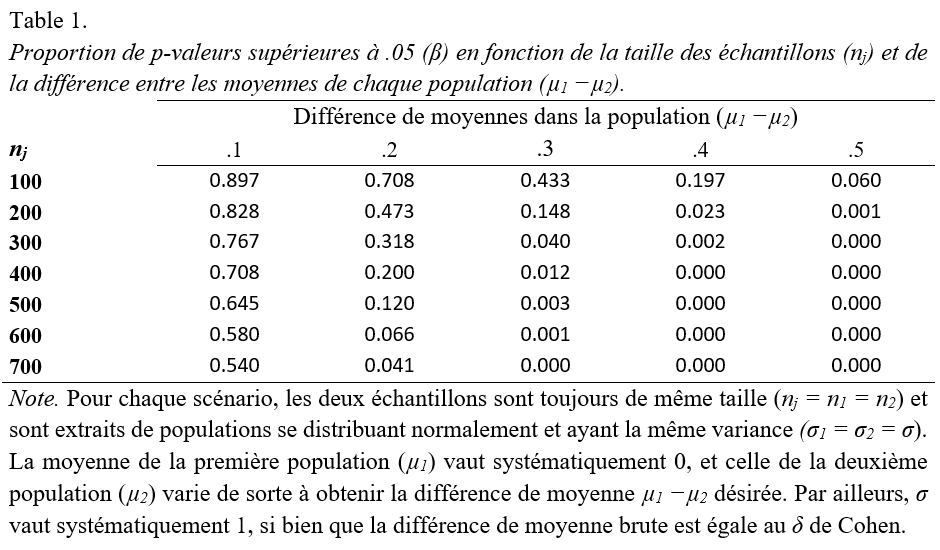
\includegraphics[width=0.95\linewidth]{C:/Users/Admin/Documents/Github projects/thesis/Chapitre 5/Illustration/Table1} \end{flushleft}
\newpage

Pour les scénarios de la première colonne, l'hypothèse nulle est vraie: il n'y a pas de différence entre les moyennes de population. Puisque les conditions d'application du test \(t\) de Student sont toutes rencontrées, on est amené à rejeter l'hypothèse nulle, c'est-à-dire à commettre une erreur de type \(I\) dans une proportion d'itération égale à \(\alpha = 5\%\). Par conséquent, on est amené à \emph{ne pas} rejeter l'hypothèse nulle \(95\%\) du temps (ce qui correspond à \((1-\alpha)\%\))\footnote{Nous observons en réalité des proportions qui varient de $94.8\%$ à $95\%$, à cause du hasard d'échantillonnage, mais sur le long terme, lorsque le nombre d'itérations tend vers l'infini, toutes les proportions ne non rejet de l'hypothèse nulle quand l'hypothèse nulle est vraie vont tendre vers $(1-\alpha) \%$.}. Pour les scénarios envisagés dans toutes les autres colonnes de la Table 1, une vraie différence entre les moyennes de population existe, si bien que le rejet de l'hypothèse nulle est la bonne décision. Pourtant, pour plusieurs scénarios, le nombre d'itérations amenant à conclure au non rejet de l'hypothèse nulle est bien supérieur au nombre d'itérations amenant à conclure au rejet de l'hypothèse nulle, comme on peut le voir à travers les valeurs \(\beta\). Par exemple, avec 100 sujets par groupes et considérant \(\sigma_1=\sigma_2=1\), on ne détectera pas une différence de moyenne de .1 dans près de 90\% des cas. Avec 700 sujets par groupe, cette différence ne sera toujours pas détectée plus d'une fois sur deux (\(\approx 54 \%\) des itérations). En présence d'un effet non nul, cela se justifie par un manque de puissance des tests réalisés, ce qui démontre bien qu'un non rejet de l'hypothèse nulle peut en fait signifier deux choses: soit qu'il n'y a vraiment pas de différence entre les moyennes des populations (ou autrement dit, que les différences observées sont dûes au hasard), soit que le test n'est pas suffisamment puissant pour détecter la différence. Or, le manque de puissance des tests est récurrent dans la littérature, comme tendent à le montrer diverses méta-analyses (\textbf{button\_power\_2013?}; \textbf{bakker\_rules\_2012?}; \textbf{funder\_improving\_2014?}).

Pour éviter d'interpréter un test peu puissant comme un soutien en faveur de l'hypothèse nulle, l'approche de la puissance est devenue l'approche par défaut dans les années 80 pour tester l'équivalence (\textbf{meyners\_equivalence\_2012?}). A travers cette approche qui est restée très populaire (\textbf{quertemont\_how\_2011?}), dans un premier temps, on définit ce qu'on considère comme étant la plus petite valeur d'intérêt (en anglais, le ``SESOI'' pour ``Smaller Effect Size of Interest''), c'est-à-dire la taille d'effet minimale requise pour considérer qu'un effet est pertinent. Ensuite, on estime la puissance de notre test à détecter un effet de cette taille\footnote{On parle d'estimation et non de mesure, car la puissance du test dépend de $\sigma$, l'écart-type de la population, qu'on ne connait pas et devra donc estimer sur base de $S$, l'écart-type de l'échantillon (Schuirmann,1987).}, et si cette estimation atteind une valeur jugée satisfaisante (en général, 80\%), alors on considère que l'on peut interpréter le non rejet de l'hypothèse nulle d'absence d'effet comme soutien en faveur de l'équivalence (\textbf{quertemont\_how\_2011?}; \textbf{meyners\_equivalence\_2012?}; \textbf{schuirmann\_comparison\_1987?}). L'idée sous-jacente est que si l'effet est au moins aussi grand que les bornes de la zone d'équivalence, sur le long terme, on devrait le plus souvent rejeter l'hypothèse nulle. Par conséquent, un non rejet de l'hypothèse nulle devrait généralement signifier que l'effet n'atteint pas le SESOI et donc, que l'effet observé n'est pas pertinent. Bien que ce raisonnement puisse sembler tentant, de prime abord, il présente d'importantes limites.

Premièrement, le test n'a pas de bonnes propriétés asymptotiques. Ceci est illustré au sein de la Table 2, dans laquelle nous envisageons les mêmes scénarios que dans la Table 1 et ajoutons une contrainte de puissance: nous décidons qu'on ne peut conclure à l'équivalence que si l'on atteind une puissance de 80\% pour détecter une différence de moyenne de .3. On constate qu'avec 100 sujets par groupes, aucune itération n'amènera à conclure à l'équivalence, pas même lorsque la différence entre les moyennes de population vaut 0. Cela s'explique par le fait que l'on n'atteind jamais la puissance minimale de \(80\%\).\footnote{Avec 100 sujets par groupe, on estime la puissance du test à $80\%$ lorsque l'estimation $d$ de Cohen vaut .3981. Par conséquent, un test sera susceptible de conclure à l'équivalence si les bornes de la zone d'équivalence, exprimée en mesure standardisée $d$ de Cohen, sont supérieures ou égales à .3981. Lorsqu'on fixe les bornes aux différences de moyennes $\pm .3$, cela n'est possible que si $S$ est inférieur ou égal à .7535. En effet, $d=\frac{\theta}{S} \leftrightarrow .3981 = \frac{.3}{S} \leftrightarrow S = \frac{.3}{.3981}=.7535$.  Or, avec 100 sujets par groupe, aucune estimation $S$ ne sera inférieure ou égale à .7535 lorsque $\sigma$ vaut 1.} Par contre, une fois les échantillons assez grands pour s'assurer une puissance de \(80\%\) pour détecter une différence de moyennes de population de .3, lorsque la différence entre les moyennes de populations est non nulle, la proportion d'itérations qui amènent à conclure à l'équivalence diminue à mesure que la taille des échantillons augmente. Par exemple, lorsque la différence de moyennes vaut .1 au niveau des populations, on conclura à l'équivalence dans \(81\%\) des itérations avec 200 sujets par groupe, contre seulement \(54\%\) des itérations avec 700 sujets par groupe \footnote{En comparant les Tables 1 et 2, on constate qu'avec 200 sujets par groupes, les proportions d'itérations de chaque scénario qui amènent à conclure à l'équivalence, dans la Table 2, sont inférieures aux proportions d'itérations de chaque scénarios qui amènent à ne pas rejeter l'hypothèse nulle, dans la Table 1. Plus les échantillons sont grands, plus la valeur maximale de $S$ permettant d'assurer la puissance des $80\%$ sera élevée. Par exemple, avec 200 sujets par groupes, la valeur maximale autorisée pour $S$ sera de $\frac{.3}{.2808}=1.07$. Avec 300 sujets par groupes, la valeur maximale autorisée pour $S$ sera de $\frac{.3}{.2291}=1.31$}.

. on sera amené à ne pas rejeter l'hypothèse nulle dans une proportion de cas inférieure à \((1-\alpha)\%\) pour le scénarios dans lequel la différence de moyennes de population est nulle. \emph{C'est vraisemblablement dû à la dispersion de la distribution d'échantillonnage de \(S\), l'estimation de l'écart-type: pour un petit nombre d'itérations, l'estimation de \(S\) serait telle que la puissance estimée serait inférieure à \(80\%\).}

car on n'atteint pas la puissance minimale requise. Une fois la puissance minimale requise atteinte, par contre, on constate que la proportion d'itérations qui amènent à conclure à l'équivalence diminue à mesure que la taille des échantillons augmente. Par exemple, si la probabilité de conclure à l'équivalence est d'environ \(81 \%\) lorsque la vraie différence de moyenne vaut .1 et qu'il y a 200 sujets par groupe, cette probabilité tombe à approximativement \(54\%\) avec 700 sujets par groupe.

\begin{flushleft}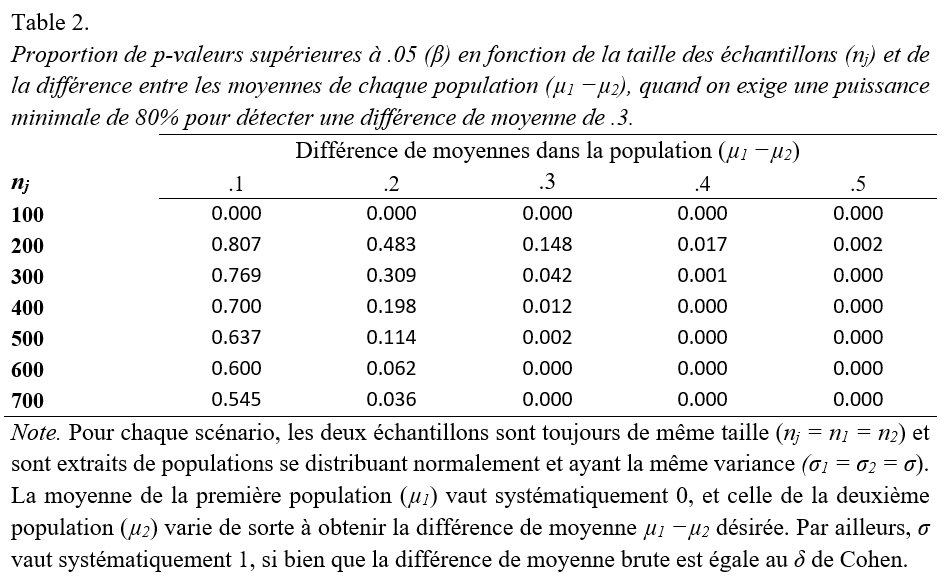
\includegraphics[width=0.95\linewidth]{C:/Users/Admin/Documents/Github projects/thesis/Chapitre 5/Illustration/Table2} \end{flushleft}

Deuxièmement, pour une taille d'échantillon donnée, plus l'erreur (la variabilité des scores au sein de chaque groupe) sera plus grande (\textbf{meyners\_equivalence\_2012?}; \textbf{schuirmann\_comparison\_1987?}), plus la probabilité de conclure à l'équivalence augmentera. Ce dernier point est illustré au sein de la Figure \ref{fig:schuirman2}, dans le contexte de la comparaison de deux moyennes. Sur l'axe des abscisses, on représente différentes estimations de la différence de moyenne (\(\bar{X_1}-\bar{X_2}\)) et sur l'axe des ordonnées, la précision des estimations \(\bar{X_1}-\bar{X_2}\) (\(S\sqrt{\frac{2}{n}}\) correspond à l'estimation de l'erreur standard de \(\bar{X_1}-\bar{X_2}\), avec \(S\) étant l'écart-type poolé et \(n\) la taille de chaque échantillon, lorsque les échantillons ont tous les deux la même taille et sont extraits de population ayant la même variance)\footnote{Par facilité, à l'instar de Schuirman (1987), on envisage le cas où les échantillons sont de même taille et que l'on suppose que la condition d'homogénéité des variances est respectée. Notons cependant que d'après Schuirman, ce raisonnement peut être généralisé aux scénarios où les deux échantillons n'ont pas la même taille et sont extraits de population n'ayant pas la même variance.}. Le triangle grisé représente l'ensemble des combinaisons estimation/précision qui vont amener à conclure à l'équivalence, avec l'approche de la puissance, lorsqu'on travaille avec des échantillons de taille 50, en acceptant un risque \(\alpha\) de 5\% et en exigeant une puissance minimale de 80\% pour détecter une différence de 20 unités (\(|\theta_j=20|,\;j=1,2\)). Dans cet exemple, pour toutes les valeurs de \(S\sqrt{\frac{2}{n}}\) supérieures à 7.07 aucune estimation de différence de moyennes ne permettra de conclure à l'équivalence (pas même 0) puisque la puissance du test à détecter une différence de 20 unités est inférieure à 80\%. Pour toutes les valeurs de \(S\sqrt{\frac{2}{n}}\) inférieures à 7.07, on constate que plus notre estimation de \(\bar{X_1}-\bar{X_2}\) est précise (lorsqu'on se déplace du haut vers le bas, sur l'axe des ordonnées), plus l'estimation doit être proche de 0 pour pouvoir conclure à l'équivalence. Comme on peut le voir à travers le triangle hachuré sur la Figure 1, cette propriété peu désirable n'est pas partagée par le TOST, un test d'équivalence que nous allons décrire ci-dessous (\textbf{schuirmann\_comparison\_1987?}).

\begin{figure}

{\centering 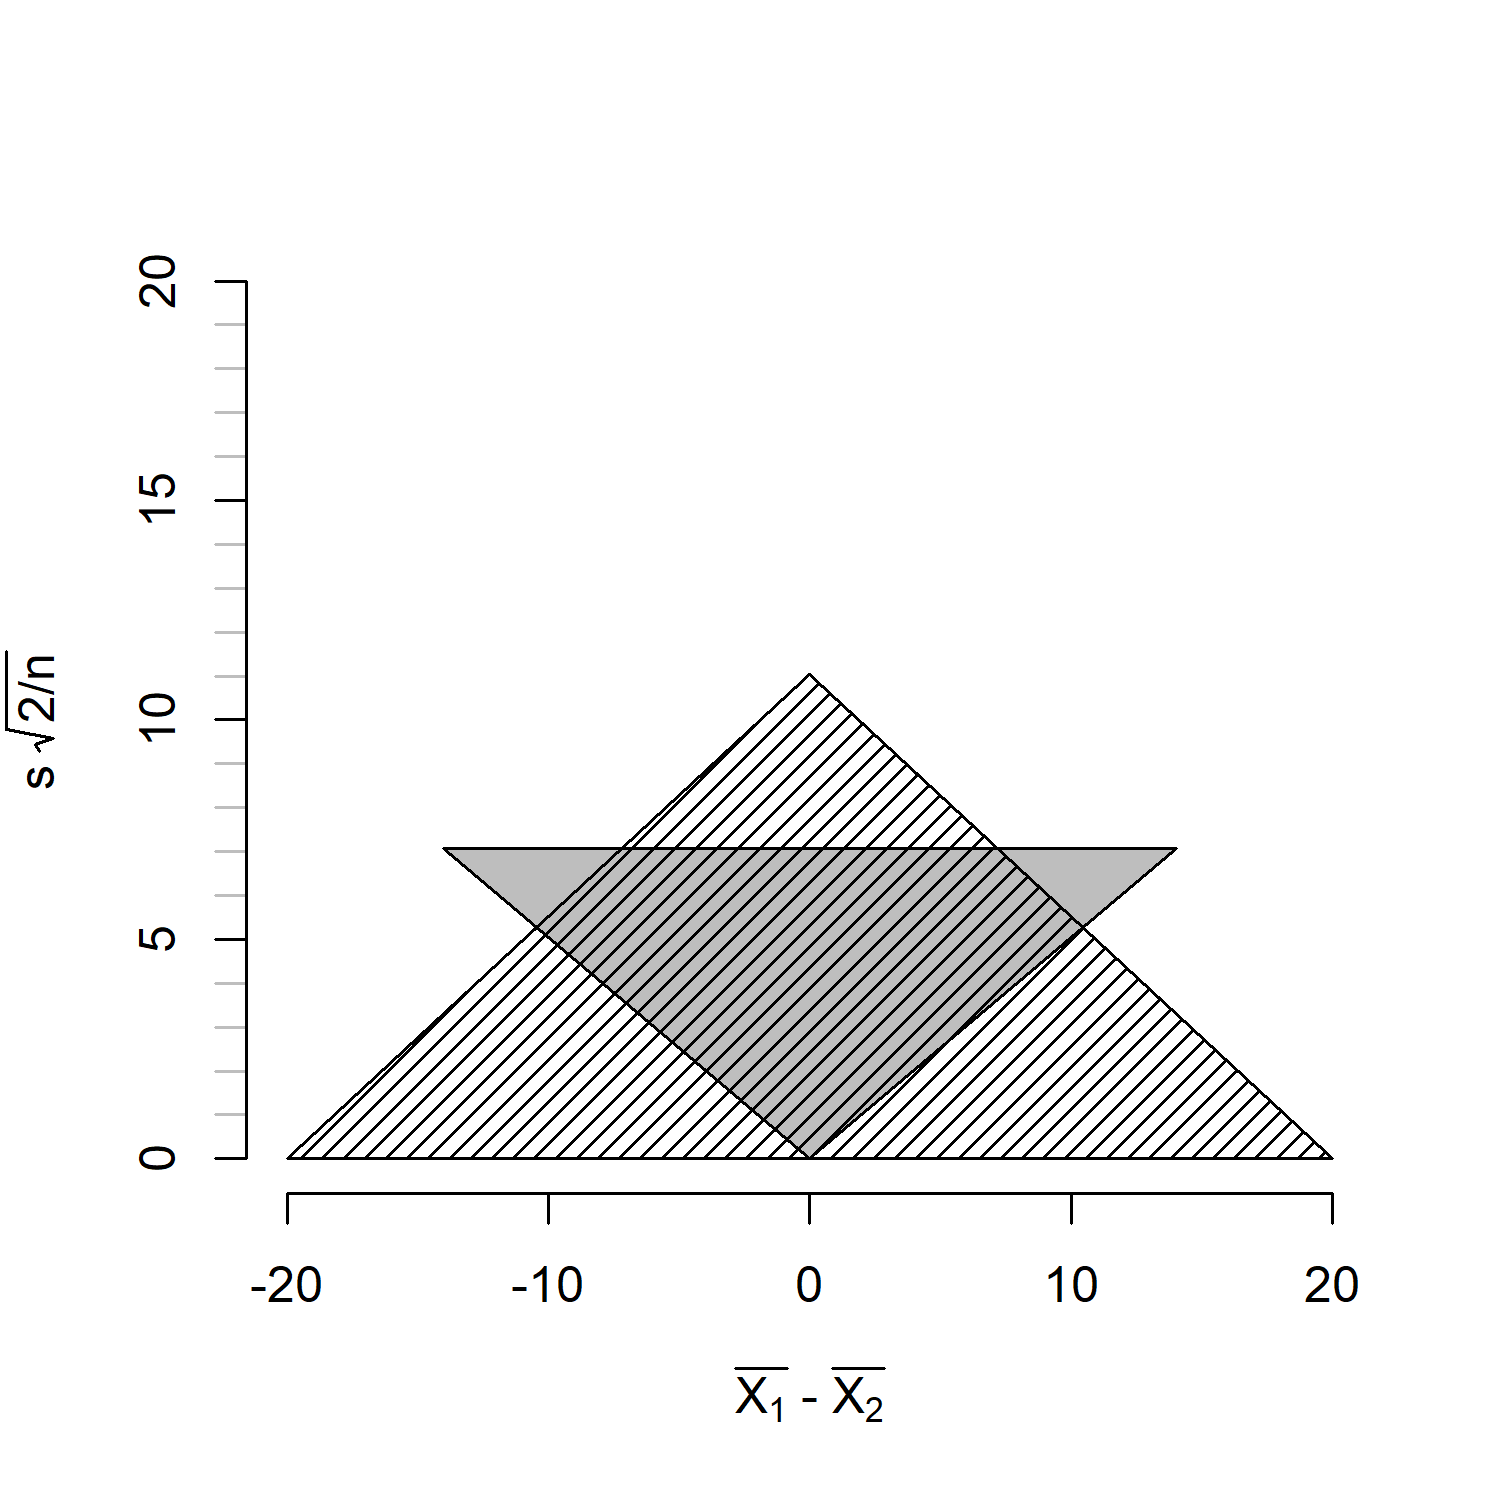
\includegraphics[width=0.6\linewidth]{C:/Users/Admin/Documents/Github projects/thesis/Chapitre 5/Illustration/Fig1} 

}

\caption{Région d'équivalence pour l'approche de la puissance (zone grisée) et pour le TOST (zone hachurée), pour l'exemple où $|\theta$|=20, n = 50 et $\alpha=.05$}\label{fig:schuirman2}
\end{figure}

\newpage

\hypertarget{les-tests-duxe9quivalence}{%
\subsection{Les tests d'équivalence}\label{les-tests-duxe9quivalence}}

Avec les tests d'équivalence, il n'est pas possible de démontrer qu'un effet vaille exactement zéro (\textbf{meyners\_equivalence\_2012?}). Il est par contre possible de montrer que l'effet observé est suffisamment petit pour être jugé non pertinent. Or, cela peut s'avérer précieux dans de nombreuses situations, par exemple pour justifier la décision de regrouper plusieurs groupes de sujets ensemble (\textbf{rogers\_using\_1993?}), pour contrôler qu'il n'y ait pas de différence trop importante entre les groupes sur base de critères autres que le (ou les) facteur(s) d'intérêts en cas de quasi-expérience (\textbf{seaman\_equivalence\_1998?}) ou encore pour falsifier une théorie qui prônerait en faveur d'un effet dépassant une certaine taille (\textbf{lakens\_equivalence\_2017?}; \textbf{anderson\_theres\_2016?}).

Le point de départ des tests d'équivalence est de définir \(\theta_1\) et \(\theta_2\), les bornes inférieures et supérieures de la zone d'équivalence, cette dernière contenant l'ensemble des valeurs jugées trop petites pour être susceptibles de nous intéresser. Ces bornes peuvent être exprimées soit dans l'unité des données brutes, soit en terme standardisé, mais doivent être définies avant la récolte des données (\textbf{anderson\_theres\_2016?}; \textbf{lakens\_equivalence\_2018?}). Il existe ensuite plusieurs approches pour démontrer que l'effet observé se situe dans la zone d'équivalence (voir \textbf{meyners\_equivalence\_2012?}, par exemple). Parmis celles-ci, une approche très simple est celle du ``Two one-sided tests'' (\textbf{schuirmann\_comparison\_1987?}; \textbf{lakens\_equivalence\_2017?}), plus communément appelé le TOST \footnote{Il existe des alternatives au TOST qui sont très légèrement plus puissantes, mais le gain marginal en termes de puissance est contrebalancé par un niveau de complexité beaucoup plus élevé (Meyners, 2012).}. Le principe est de définir deux hypothèses nulles. La première est que l'effet observé est inférieur à la borne inférieure de la zone d'équivalence: \[\it H0_1: \theta < \theta_1, \; avec \; \theta_1 \neq 0\] La deuxième est que l'effet observé est supérieur à la borne supérieure de la zone d'équivalence: \[\it H0_2: \theta > \theta_2, \; avec \; \theta_2 \neq 0\] Lorsque les deux hypothèses nulle peuvent être simultanément rejetées, on peut conclure à l'équivalence (\textbf{seaman\_equivalence\_1998?}). Cela équivaut, statistiquement parlant, à montrer que l'intervalle de confiance à \((1-2\times\alpha)\%\) est entièrement inclus dans la zone d'équivalence (\textbf{seaman\_equivalence\_1998?}; \textbf{lakens\_equivalence\_2017?}). Notons qu'il n'est pas nécessaire de reporter les résulats des deux tests unilatéraux, lorsqu'on réalise le TOST: il suffit de reporter les résultats du test associé à la plus petite valeur de statistique (et par conséquent, à la plus grande \(p\)-valeur). En effet, si ce test amène à conclure au rejet de l'hypothèse nulle, le second test amènera automatiquement à la même conclusion (\textbf{rogers\_using\_1993?}; \textbf{lakens\_equivalence\_2018?}). Cette remarque reste vraie dans le cas particulier où les deux tests sont associés à la même valeur de statistique puisque dans ce cas, les deux tests mèneront à une conclusion identique (\textbf{rogers\_using\_1993?}). Notons également qu'il n'est pas nécessaire de procéder à une correction du risque alpha dûe à la réalisation simultanée de deux tests. En effet, une erreur de type \(I\) (rejeter à tort l'hypothèse nulle) ne peut être commise que si l'hypothèse nulle est vraie. Or, les deux hypothèses nulles testées sont mutuellement exclusives: il n'est pas possible que \(\theta\) soit simultanément inférieur à \(\theta_1\) (ce qui correspond à \(\it H0_1\)) et supérieur à \(\theta_2\) (ce qui correspond à \(\it H0_2\)).

Jusqu'il y a peu, le TOST n'était pas disponible dans la plupart des logiciels, à l'exception de Minitab, ce qui constituait un frein important à son usage. Pour cette raison, (\textbf{lakens\_20\_2016?}) a créé le package R ``TOSTER'' et plus récemment encore, ce même package a été implémenté dans Jamovi \footnote{Jamovi est un logiciel clic-bouton entièrement gratuit qui gagne en popularité et qui présente, parmi ses nombreux avantages, le fait d'être particulièrement convivial. Dans la mesure où la plupart des chercheurs sont plus enclins à utiliser des procédures si elles sont implémentées dans ce type de logiciel (Fraas $\&$ Newman, 2000), cela constitue une excellente nouvelle pour le devenir du TOST dans la recherche en psychologie.}. Tant dans R que dans Jamovi, le package compare simultanément l'effet observé à l'absence d'effet (cela correspond au test traditionnel) ainsi qu'aux deux bornes de la zone d'équivalence (cela correspond au TOST). Il en découle 4 conclusions distinctes possibles (\textbf{lakens\_equivalence\_2017?}), qui sont illustrées dans la figure \ref{fig:equiv1} dans le contexte de la comparaison de deux moyennes indépendantes:

\begin{figure}

{\centering 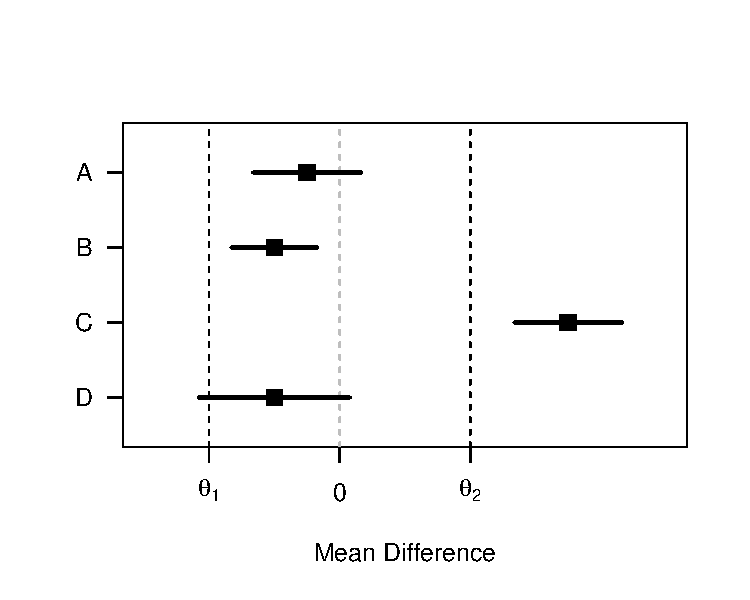
\includegraphics[width=0.8\linewidth]{chp5_files/figure-latex/equiv1-1} 

}

\caption{Différence de moyennes ($\bar{X_1}-\bar{X_2}$) et IC à $1-2\alpha\%$ autour de la différence de moyennes ($\bar{X_1}-\bar{X_2}$) pour 4 scénarios distincts.}\label{fig:equiv1}
\end{figure}

\begin{enumerate}
\def\labelenumi{(\arabic{enumi})}
\item
  La différence de moyenne observée diffère significativement des deux bornes d'équivalence, mais pas de 0 (scénario A, Figure \ref{fig:equiv1}): dans ce cas, on conclura à l'absence d'un effet au moins aussi grand que les bornes d'équivalence.
\item
  La différence de moyenne observée diffère significativement des deux bornes d'équivalence ainsi que de 0 (scénario B, Figure \ref{fig:equiv1}): on conclura alors qu'il existe un effet non nul, mais qui ne dépasse pas une certaine taille fixée par les bornes. C'est ce qui arrive typiquement lorsqu'on travaille avec de très grands échantillons, si bien que le test traditionnel est très puissant, même pour détecter des effets très petits (\textbf{rogers\_using\_1993?}).
\item
  La différence de moyenne observée diffère significativement de 0, mais ne diffère pas significativement d'au moins une des deux bornes d'équivalence (scénario C, Figure \ref{fig:equiv1}): on conclura alors à la présence d'un effet non nul (\textbf{rogers\_using\_1993?}).
\item
  La différence de moyenne observée ne diffère significativement ni d'au moins une des deux bornes d'équivalence, ni de 0 (scénario D, Figure \ref{fig:equiv1}): c'est ce qui arrive lorsque les données sont si imprécises qu'on ne peut tirer aucune conclusion. Les données semblent compatibles tant avec un effet nul qu'avec un effet supérieur au SESOI.
\end{enumerate}

\hypertarget{duxe9finir-les-bornes-de-la-zone-duxe9quivalence}{%
\subsection{Définir les bornes de la zone d'équivalence}\label{duxe9finir-les-bornes-de-la-zone-duxe9quivalence}}

L'aspect le plus compliqué dans la réalisation du TOST est la définition des bornes d'équivalence. Dans certains cas, il est possible de définir un critère objectif qui permettra de déterminer à partir de quand un effet est jugé pertinent (\textbf{lakens\_equivalence\_2018?}). Dans ce cas, établir l'équivalence revient à rejeter la présence d'un effet ayant un quelconque intérêt pratique (\textbf{rogers\_using\_1993?}). Par exemple, (\textbf{burriss\_changes\_2015?}) avaient émis l'hypothèse qu'une augmentation de la rougeur de la peau chez femmes les rendraient plus attractives pour les hommes en période d'ovulation. Or, une telle hypothèse n'est crédible que si le changement facial est visible à l'oeil nu. Dans ce contexte, le SESOI serait la plus petite variation dans la rougeur de la peau qu'il est possible de détecter à l'oeil nu (\textbf{lakens\_equivalence\_2018?}). Il est également parfois possible pour des experts de déterminer expérimentalement ce qui constitue un changement important, pour certaines échelles de mesures fréquemment utilisées en psychologie, à l'instar de (\textbf{button\_minimal\_2015?}) qui se sont penchés sur le BDI\footnote{Le BDI (Beck Depression Inventory) est une échelle auto-rapportée évaluant les symptômes cognitifs courants de la dépression.  Cette échelle est constituée de 21 items évalués à l'aide des échelles de Likert allant de 0 à 3, ce qui donne un score total compris entre 0 et 63 qui sera d'autant plus élevé que la dépression sera sévère (Button et al., 2015).}. Ces auteurs ont interrogé un grand nombre de patients quant à leur ressenti subjectif en termes d'amélioration de leur dépression dans un certain laps de temps, et ont comparé leurs réponses à la différence de score obtenu à l'aide du BDI dans ce même laps de temps (\textbf{lakens\_equivalence\_2018?}).

Malheureusement, il n'est pas toujours possible d'établir un critère objectif en vue de définir les bornes d'équivalence. Dans ce cas, il existe diverses stratégies, plus subjectives, en vue d'établir ces bornes. En les utilisant, il faut cependant avoir conscience du fait que la question à laquelle nous répondons varie en fonction de la stratégie utilisée.

Premièrement, il est possible de déterminer des bornes en s'inspirant de balises existantes, en vue d'exclure la présence d'un effet jugé petit, moyen ou grand par ces balises (\textbf{lakens\_equivalence\_2018?}). Notons que si cette stratégie est tentante de par sa simplicité, elle doit être utilisée avec prudence. D'abord, un effet ne devrait être qualifié de petit, moyen ou grand qu'en comparaison à d'autres effets connus, et non sur base d'impressions qualitatives (\textbf{gignac\_effect\_2016?}). Dit autrement, il est important d'avoir un cadre de référence pour juger de la taille d'un effet. Or, les balises de Cohen (en l'occurence, les balises les plus célèbres et les plus largement utilisées) sont dépourvues de ce cadre de référence, puisqu'elles ont été établies à une époque où très peu de chercheurs se préoccupaient de la taille des effets étudiés (\textbf{funder\_evaluating\_2019?}). Depuis Cohen, certains chercheurs ont déployé de gros efforts en vue d'établir de nouvelles normes sur base d'analyses systématiques quantitative de la litérature. (\textbf{gignac\_effect\_2016?}), par exemple, ont établi de nouvelles balises pour interpréter le \(r\) de Pearson, en définissant les quartiles d'une distribution de 708 mesures dérivées de méta-analyses issues de la psychologie sociale et de la personnalité. C'est de la sorte qu'ils ont proposé d'interpréter respectivement des mesures de 0.10, 0.20 et 0.30, dans ces domaines de la psychologie, comme représentant des effets relativement petits, typiques et relativement larges. Ces normes ont également été approuvées par (\textbf{funder\_evaluating\_2019?}). Ensuite, les balises ne prennent pas en compte le contexte de l'étude si bien que statuer sur la taille d'un effet ne fournit pas nécessairement d'information sur sa valeur. \emph{Un effet même de très petite taille peut faire une différence pour les personnes concernées. Yzerbit donne l'exemple suivant: l'effet de l'aspirine sur l'espérance de vie est minimale, mais pour les gens qui survivent, ça fait une différence.}. \emph{Autre exemple: Imaginons un médicament contre la dépression qui permettrait de réduire les symptômes un tout petit peu mais qui ne coûte presque rien. Une faible différence d'un point de vue statistique peut devenir une grande différence pour les personnes concernées. Idem pour un médicament qui sauve des vies}. C'est pour cette raison que les balises devraient toujours être utilisées en dernier recours, lorsqu'on ne dispose d'aucune information contextuelle.

Deuxièmement, dans le contexte d'études de réplication, il est possible de se baser sur les résultats d'études antérieures pour définir les bornes d'équivalence.
2.1. (Levine et al.~2007): se baser sur les tailles d'effet suggérées dans la littérature (sur base de méta-analyses)\footnote{Il est mieux de se baser sur des résultats de méta-analsye que d'étude isolée parce qu'à cause du biais de publication, les tailles d'effet observées sont souvent une sur-représentation de la réalité et donc si on a bcp de sujets dans notre étude, il y a vraiment bcp de chance qu'on démontre l'équivalence}.\emph{Prenons l'exemple de l'augmentation de la pensée agressive quand on joue à des jeux violents. D'après une méta-analyse de Ferguson (2007), cette corrélation serait de r =.25 (ce qui correspond à un d de Cohen de .51). Je peux utiliser cette valeur comme borne pour définir l'intervalle d'équivalence. Si je parviens à montrer qu'il y a équivalence, je montre que l'effet étudié serait vraisemblablement plus petit que suggéré dans la littérature. }.\\
--\textgreater{} Remarque: la méta-analyse elle donne .25, OK, mais en réalité, il y a une distribution autour de l'effet dans la littérature. Une solution plus conservatrice est alors de se baser sur les bornes inférieures de l'IC autour de la valeur de la méta-analyse.
--\textgreater{} Comme dit Vincent, c'est la réalité de l'effet. C'est comme si tu faisais un test entre deux moyennes en prétendant que la myenne est une valeur et pas une distribution autorud e cette effet. Et donc c'est un peu délicat d'aller dire qu'on va tester un test d'équivalence pour contester l'effet de la violence en prenant la valeur obtenue dans la méta analyse comme une borne absolue et pas une distribution. Du coup, au minimum il essayerait d'intégrer le fait qu'il y a une distribution autour de la valeur, mais donc on ne peut pas décider que si on est en dessous de .50 ou au dessus de -.50.\\
--\textgreater{} Autre probleme, pourquoi prendre l'opposé comme borne inférieure? Alors que la méta analyse ne parle pas d'effet inverse.
--\textgreater{} Pour l'heure, je serais plus d'avis de confirmer la méta-analyse en montrer que l'effet est bien situé à l'intérieur des bornes de l'IC autour de cet effet dans la méta-analyse.
2.2. Solution proposée par Simonsohn (2015) pour remettre en question la pertinence de l'outil qui a ét utilsié pour démontrer un effet dans une étude antérieure. Il dit que si on a pour un effet d'intérêt une puissance inférieure à 33\% de le détecter, on a vraiment un gros problème de puissance (pourquoi 33\% ça reste arbitraire, of course). il part de cette optique là et il se dit que du coup, ça pourrait être intérssant de définir les bornes de la zone d'équivalence en considérant un effet que l'étude d'origine aurait pu détecter avec une puissance de 33\%. Ce faisant, si on parvient à démontrer que l'effet est encore plus petit qu'un effet que l'étude ne base n'aurait pu détecter qu'avec une puissance de 33\%, il y a peu de chance pour que l'effet originellement proposé par l'étude d'origine soit vraiment basé sur un outil pertinent. \emph{exemple concrêt: imaginons un test t de Student et qu'on a 21 sujets par groupe. On peut déterminer, en faisant une analyse de sensibilité dans Gpower, qu'on a une puissance 33\% à détecter un effet d de COhen de .48. Du coup, on considererais .48 comme valeur pour notre zone d'équivalence.}\\
2.3. Lakens (2018): essayer de deviner implicitement ce que l'auteur de l'étude d'origine aurait pu considérer comme un effet pertinent (s'il n'a pas donné d'indication dans son article pour dire " je considère qu'un effet est pertinent à partir de telle valeur"). Cela peut se faire sur base de la taille d'échantillon utilisée par cette personne. \emph{On ne pourra détecter un effet comme significatif que si la valeur de statistique observée dépasse une valeur seuil (la valeur critique). Il est possible, grâce à la relation qui existe entre la statistique t et la statistique d de Cohen, de déterminer à quelle ``taille d'effet critique'' correspond la statistique t critique. Par exemple, si le chercheur a utilisé 30 sujets par groupe: via gpower, on peut déterminer qu'il faudra une statistique observée t de minimum 2.045 pour pouvoir conclure au RH0. et compte tenu du lien entre la statistique t et la stat d, ça correspond à un d de Cohen de .373 (d\_crit = t\_crit/racine(n)). Concrètement, si on observe une taille d'effet supérieure ou égale à .373, on pourra conclure au rejet de l'H0. Si la taille d'effet est plus petite, on ne sera pas capable de conclure au rejet de l'hypothèse nulle. L'idée ce serait de démontrer qu'il y a équivalence, la personne qui a écrit l'article d'origine a utilisé une taille d'échantillon insuffisante pour étudier l'effet suggéré et donc, si on veut étudier ce même sujet d'étude, il faudrait nécessairement récolter des échantillons plus grands pour être capable de le faire correctement. }

\begin{enumerate}
\def\labelenumi{\arabic{enumi})}
\setcounter{enumi}{2}
\tightlist
\item
  de se baser sur les ressources dont on dispose (analyse de sensibilité). Si moi je ne suis pas capable d'avoir un échantillon de plus de 2000 personnes, il y a certains effets que je ne serai pas capable de calculer. Et donc, je peux utiliser cette taille d'échantillon pour déterminer la taille d'effet dont je suis certain que je pourrai raisonnablement conclure au rejet de l'hypothèse nulle. Et donc là, si on démontre qu'il y a équivalence, on ne tire pas la ccl que l'effet n'est pas pertinent, mais que cet effet qu'on a envie d'étudier ne peut être l'être sur base des tailles d'échantillon qu'on a l'habitude d'utiliser.
\end{enumerate}

Il est important de bien comprendre qu'en fonction de la stratégie utilisée, on ne se posera pas nécessairement la même question de recherche (et la réponse obtenue sera nécessairement liée à cette question de recherche).

\begin{enumerate}
\def\labelenumi{\arabic{enumi})}
\tightlist
\item
  définir comme limites la plus petite taille d'effet pour laquelle on peut atteindre une puissance de détection suffisante (déterminé par les ressources disponibles pour étudier l'effet, (\textbf{lakens\_equivalence\_2017?})) --\textgreater{} voir la section ``Setting equivalence bounds'' p.~359 mais je crois que j'en parle aussi dans la vidéo SOCLAB.\\
\item
  le SESOI peut parfois être fixé objectivement
\item
  Idéalement basé sur une analyse coût-bénéfice). Attention: bien sûr une dimension subjective dans la définition des coûts et des bénéfices.
  Attention: le SESOI doit être déterminé AVANT et INDEPENDAMMENT des données.
\end{enumerate}

\hypertarget{comparaison-du-tost-et-du-sgpv}{%
\subsection{Comparaison du TOST et du SGPV}\label{comparaison-du-tost-et-du-sgpv}}

\begin{center}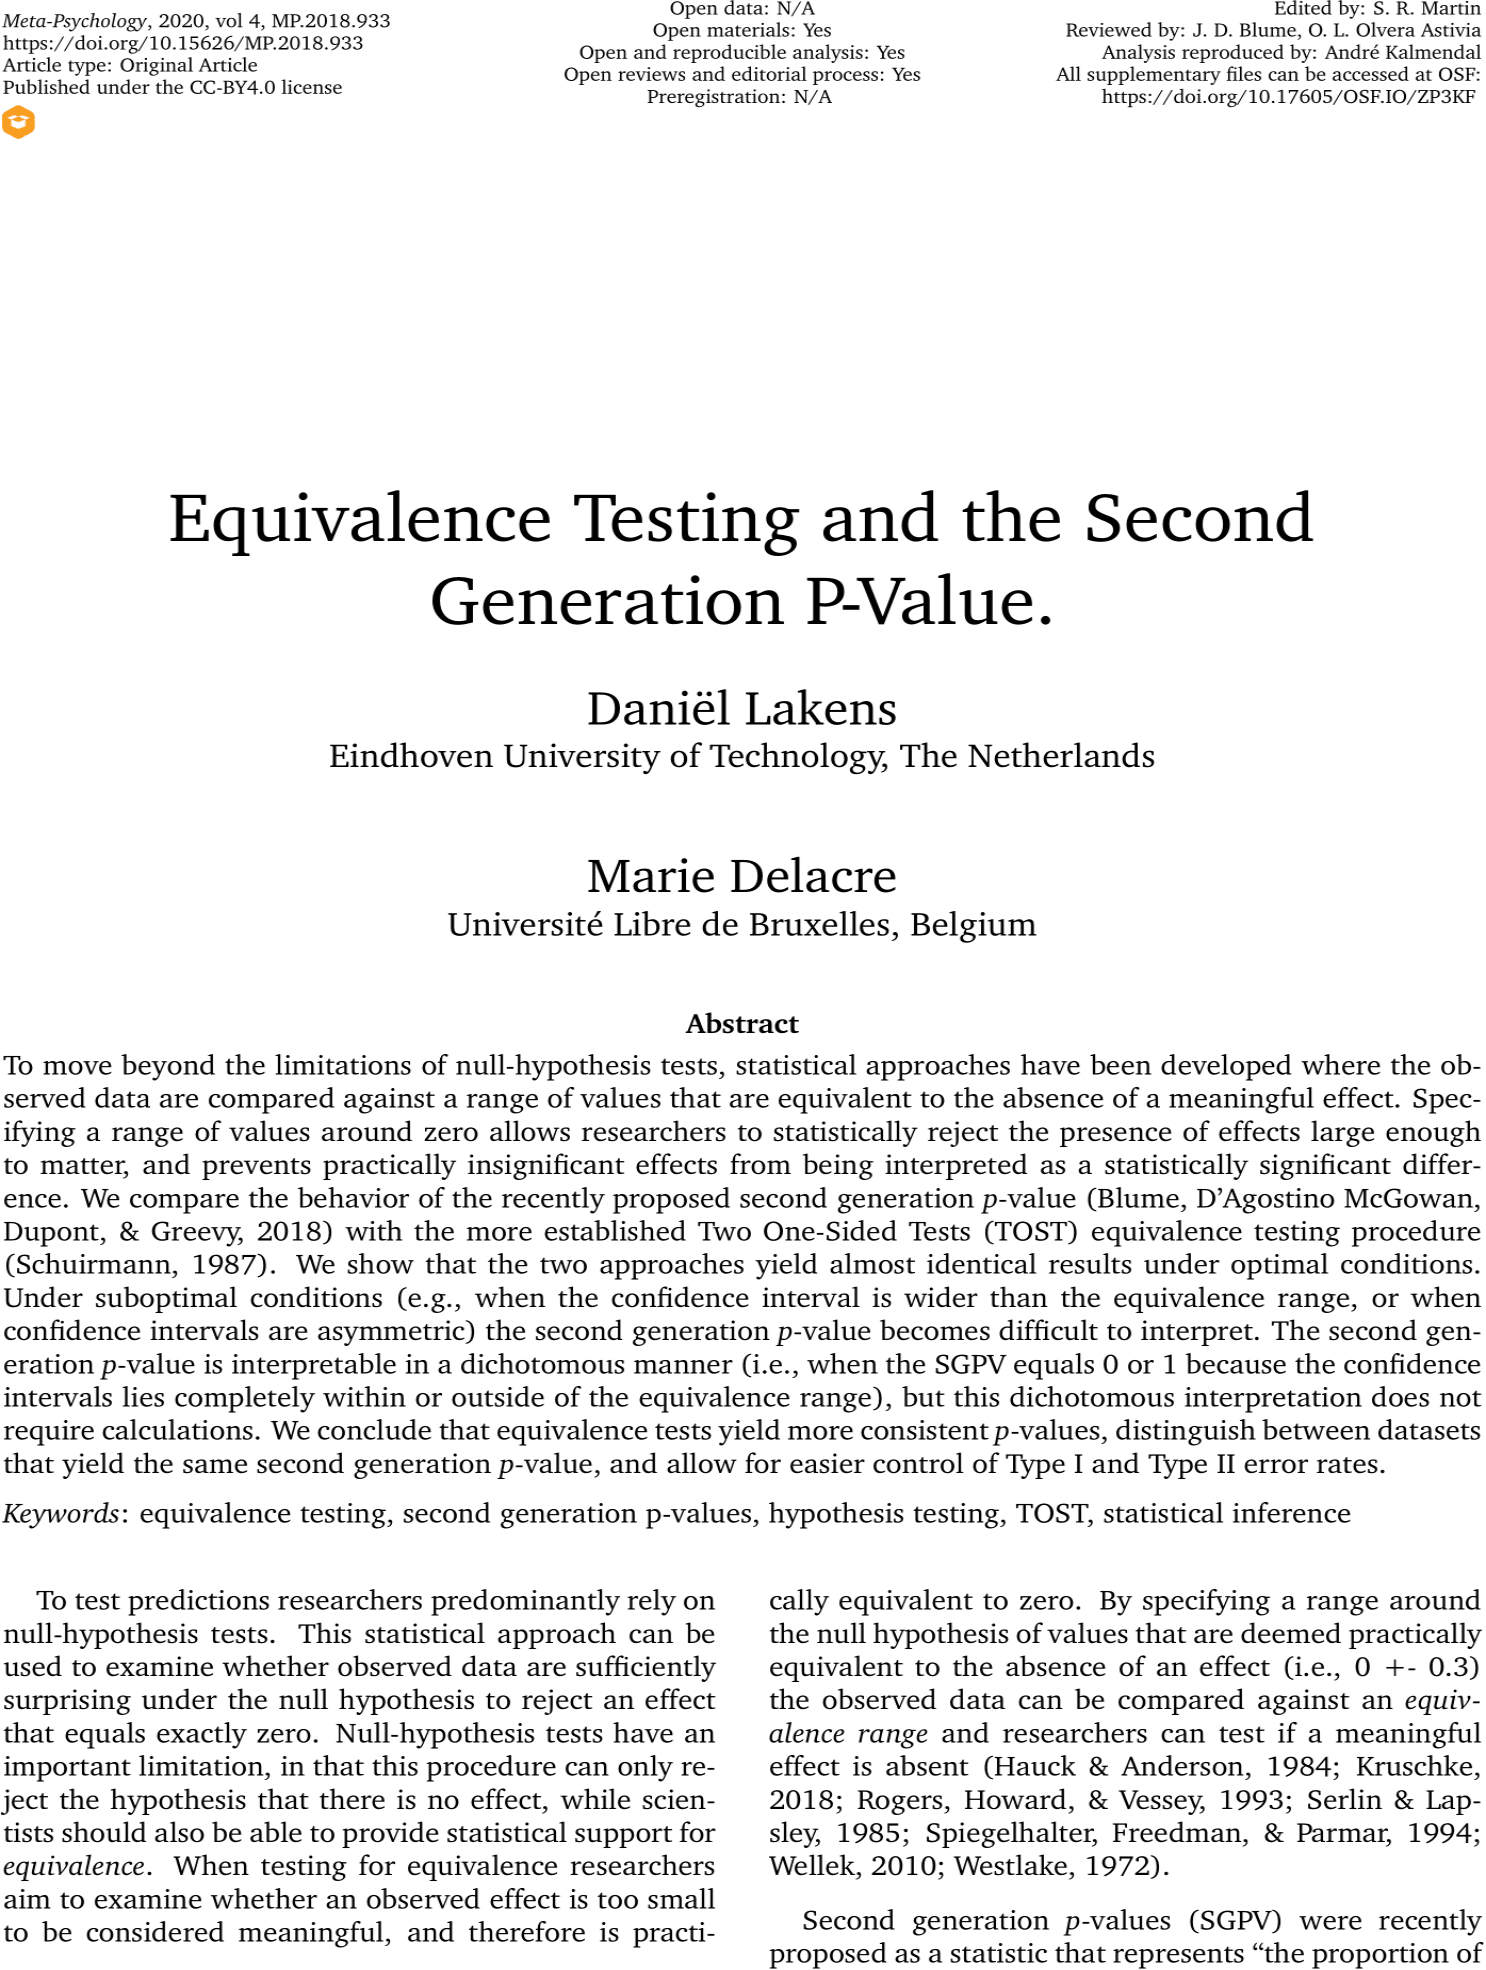
\includegraphics[width=0.92\linewidth]{C:/Users/Admin/Documents/Github projects/thesis/Chapitre 5/Chapitre 5-1} \end{center}

\begin{center}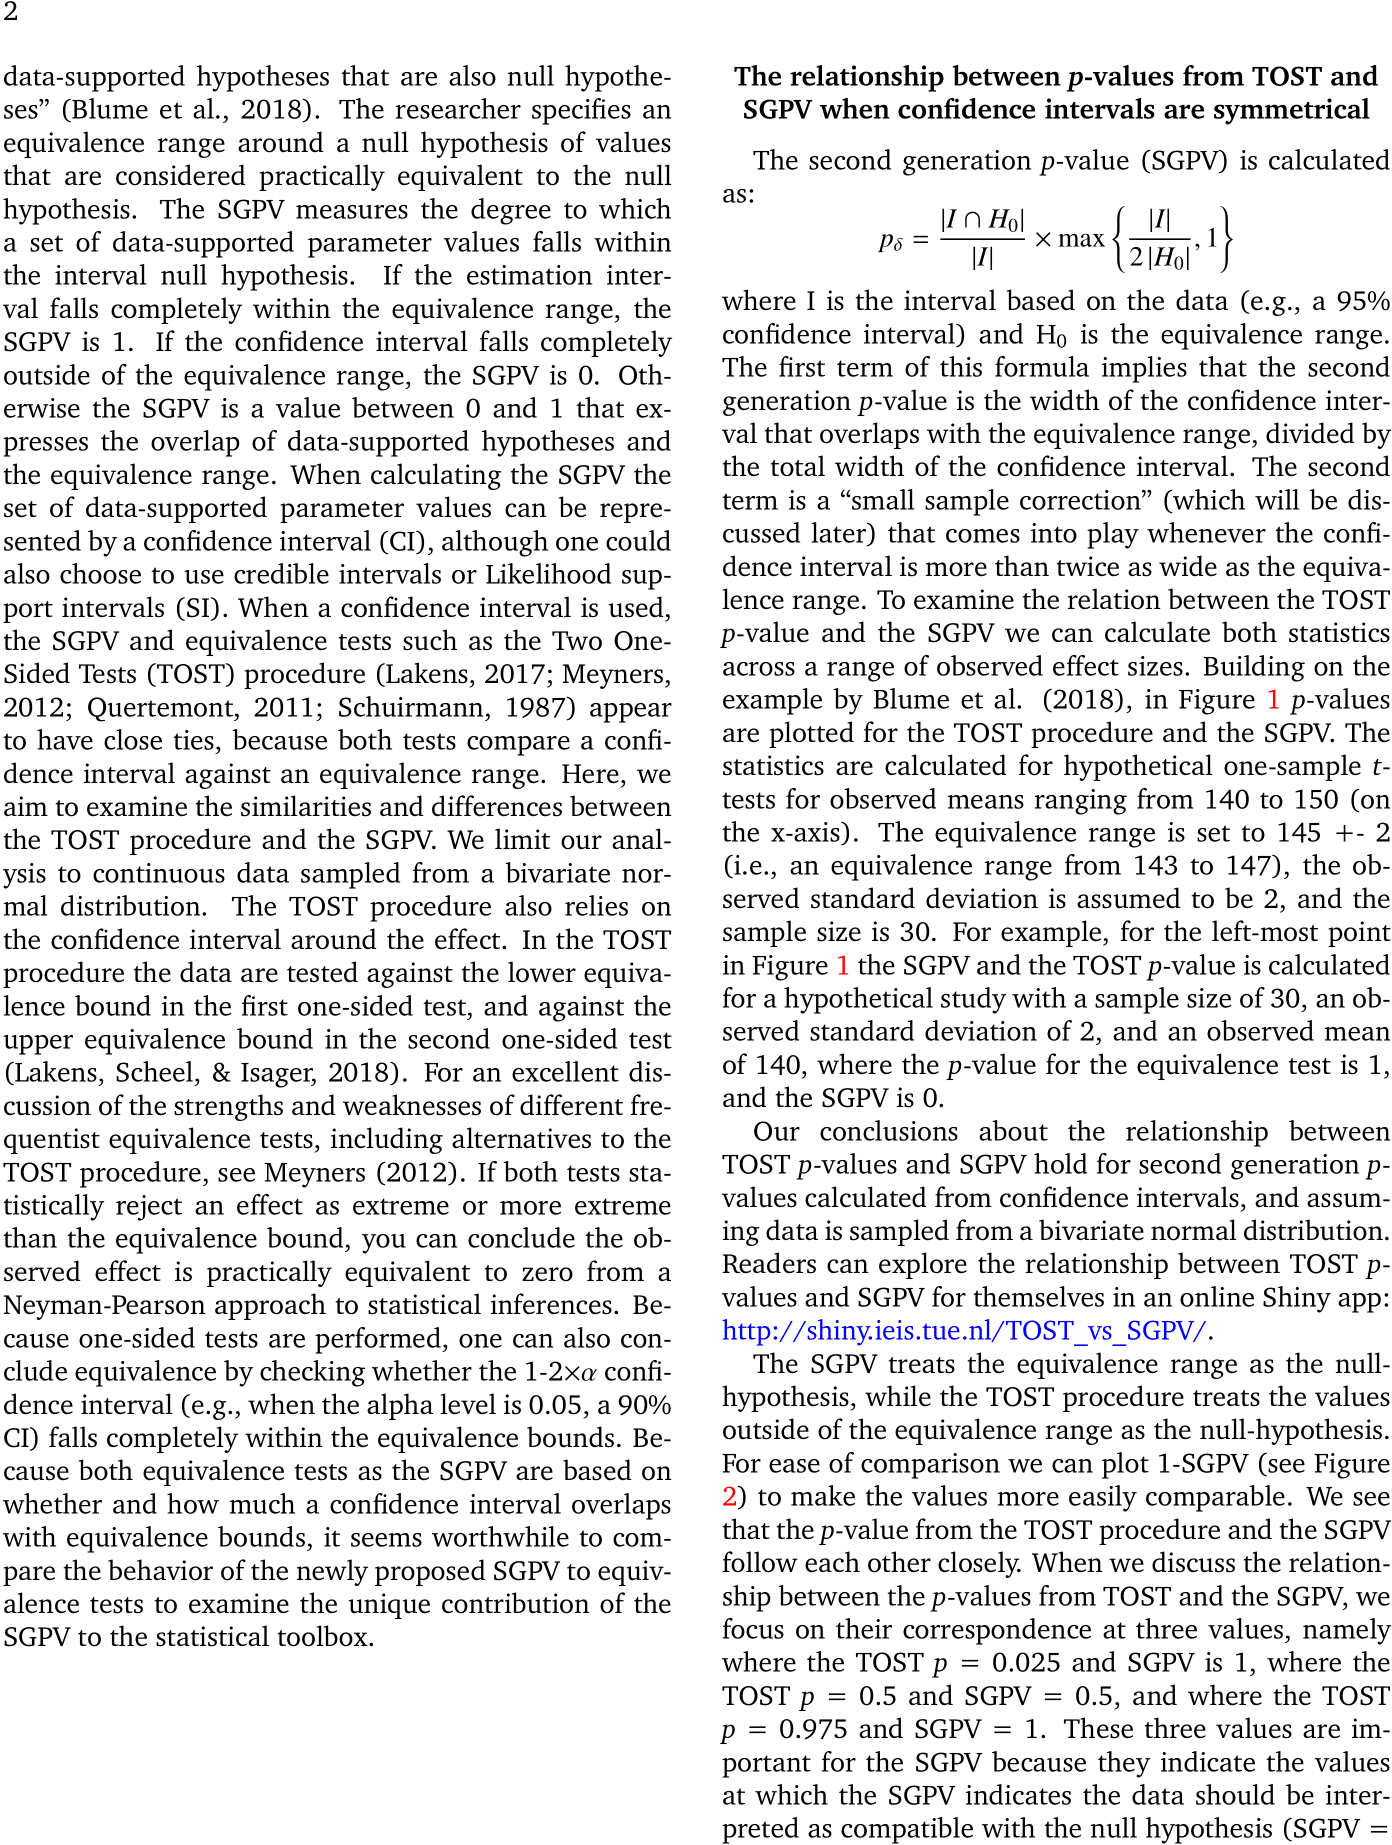
\includegraphics{C:/Users/Admin/Documents/Github projects/thesis/Chapitre 5/Chapitre 5-2} \end{center}

\begin{center}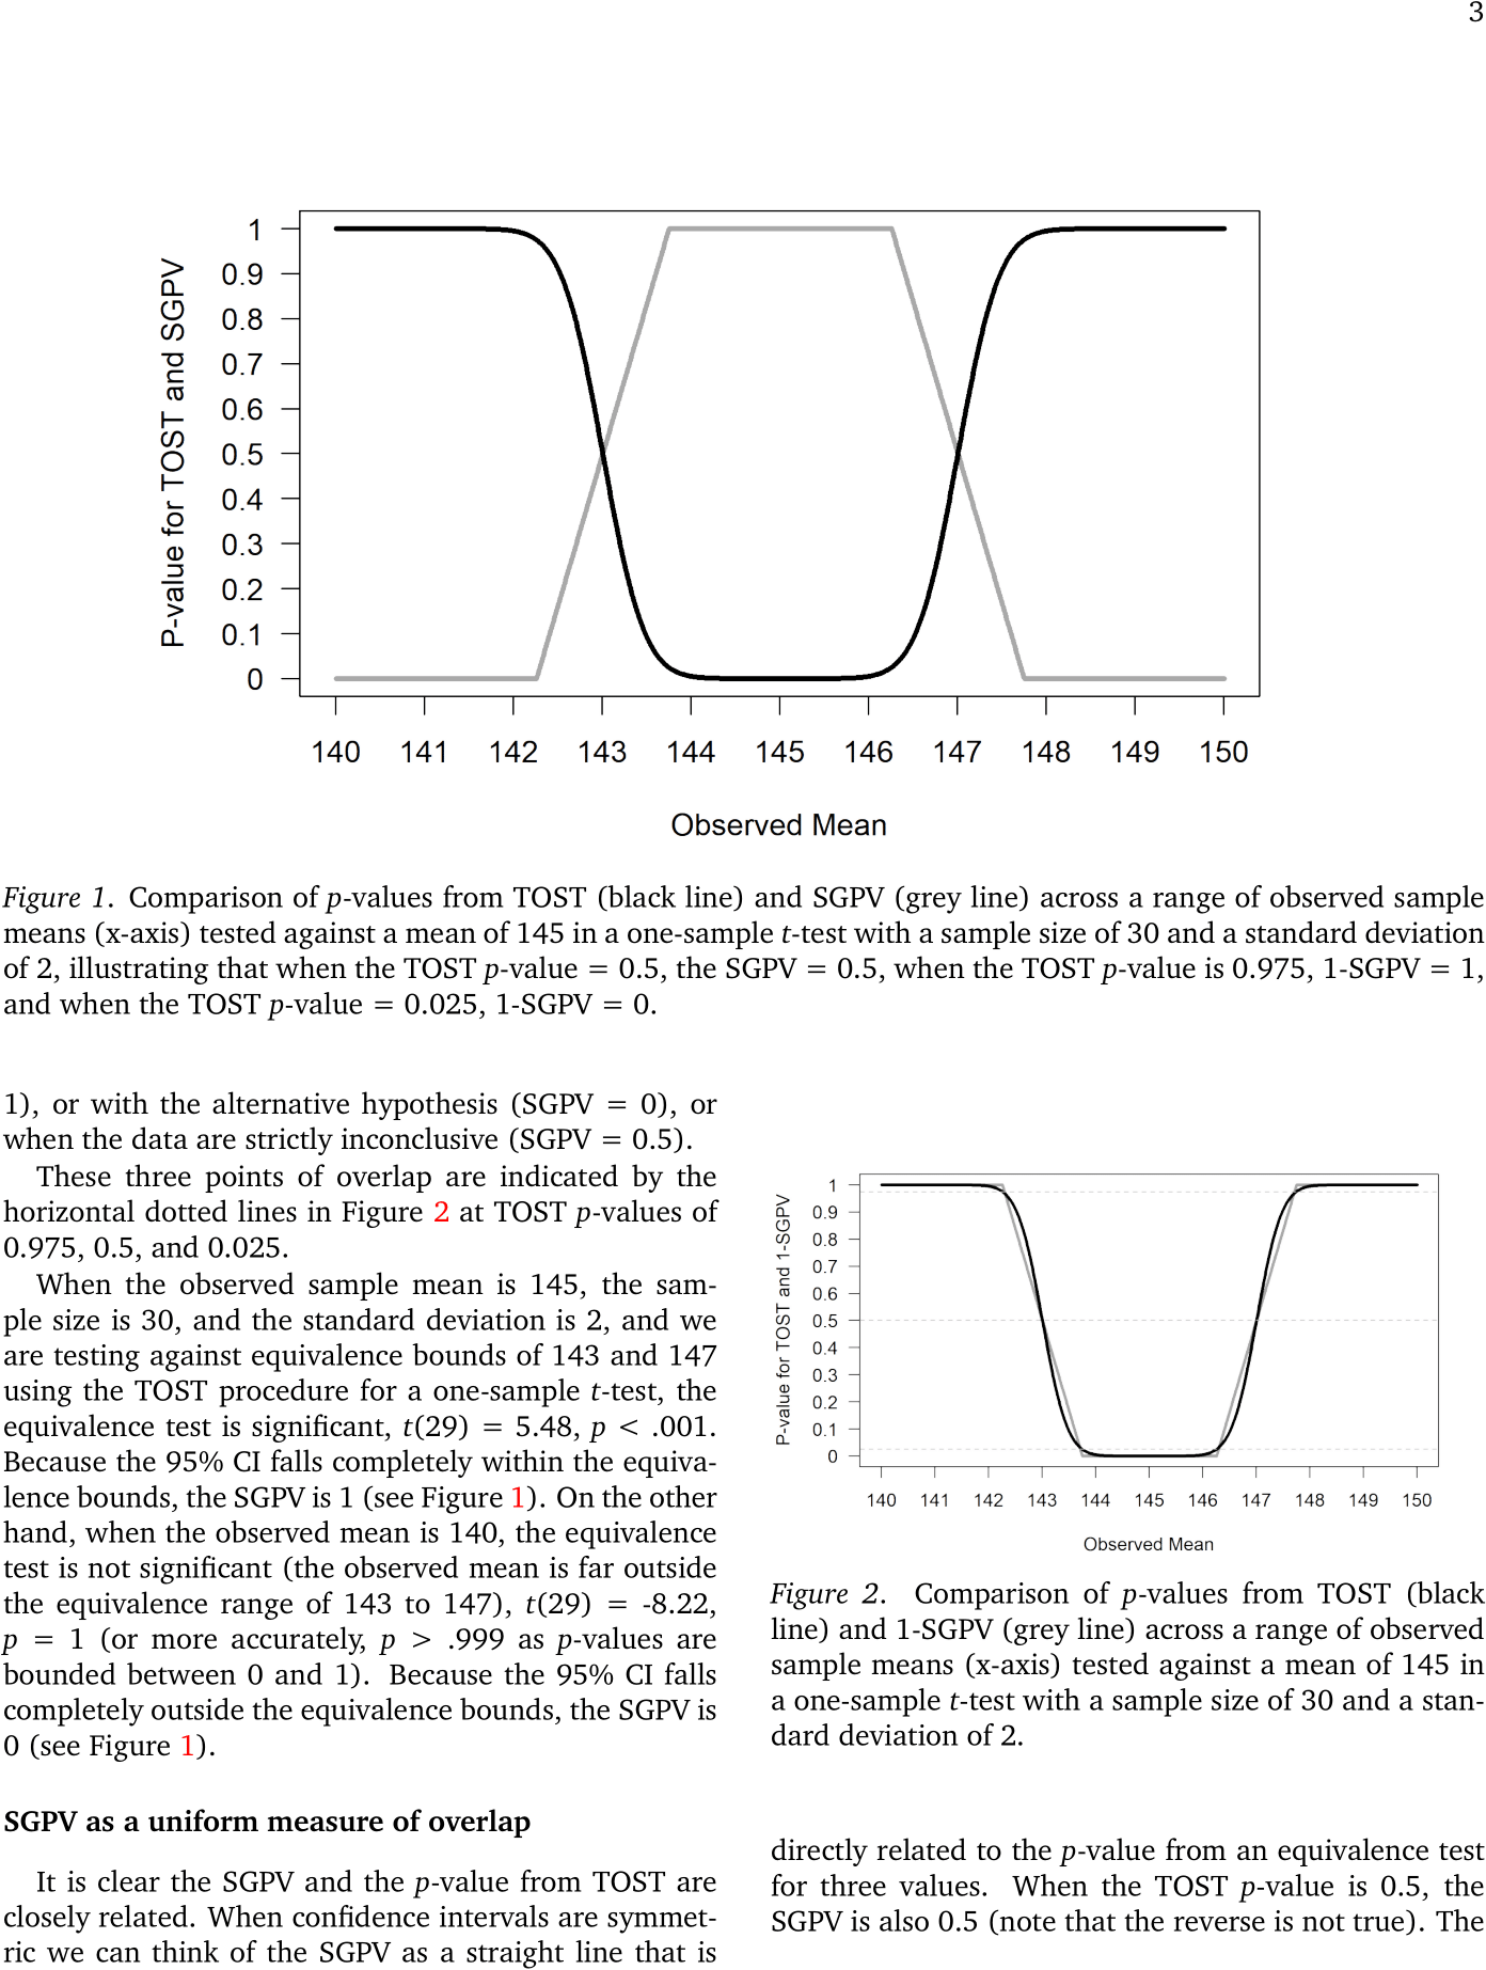
\includegraphics{C:/Users/Admin/Documents/Github projects/thesis/Chapitre 5/Chapitre 5-3} \end{center}

\begin{center}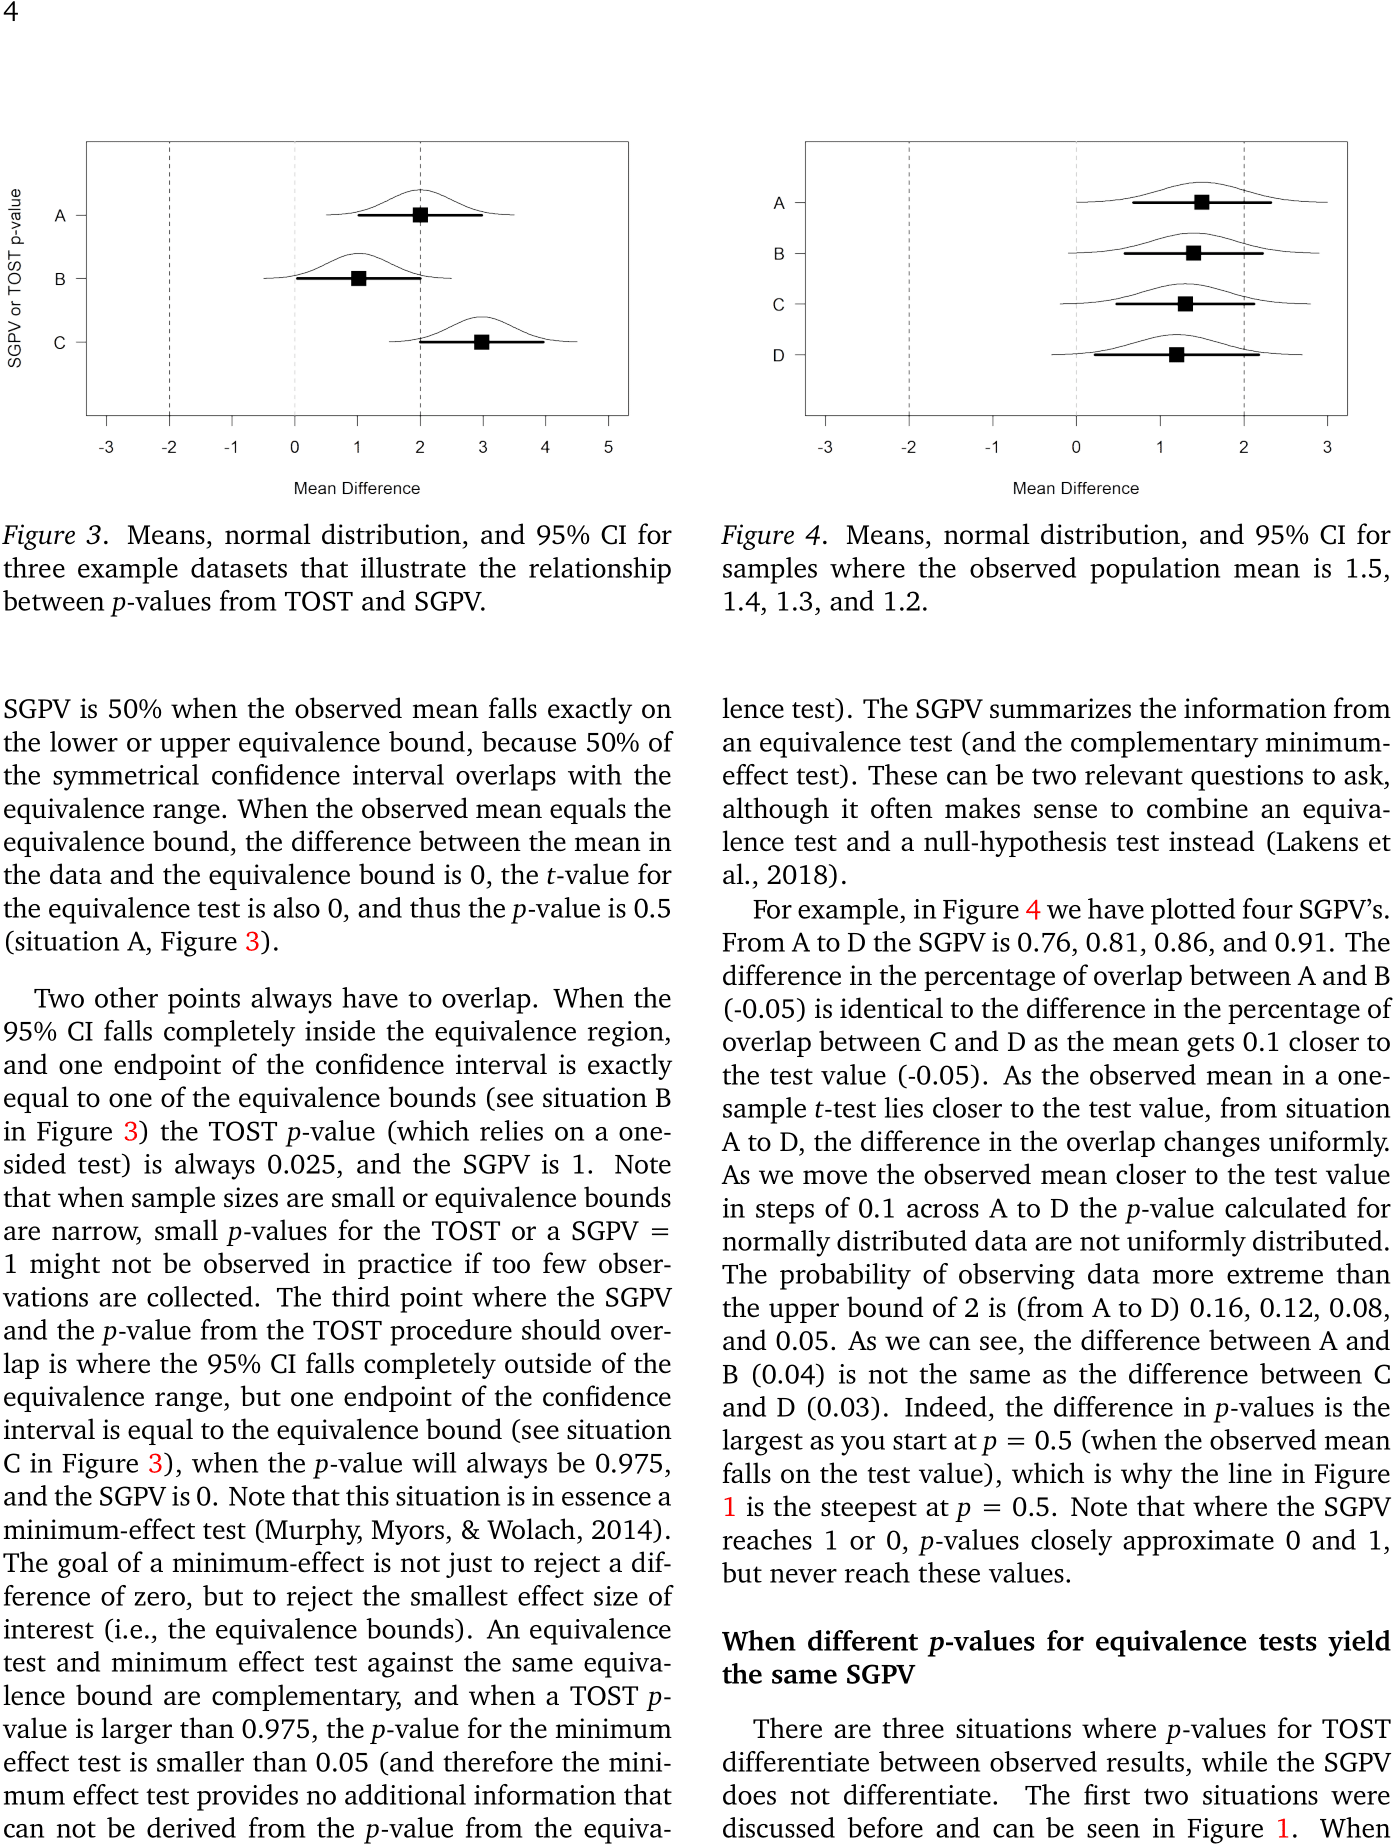
\includegraphics{C:/Users/Admin/Documents/Github projects/thesis/Chapitre 5/Chapitre 5-4} \end{center}

\begin{center}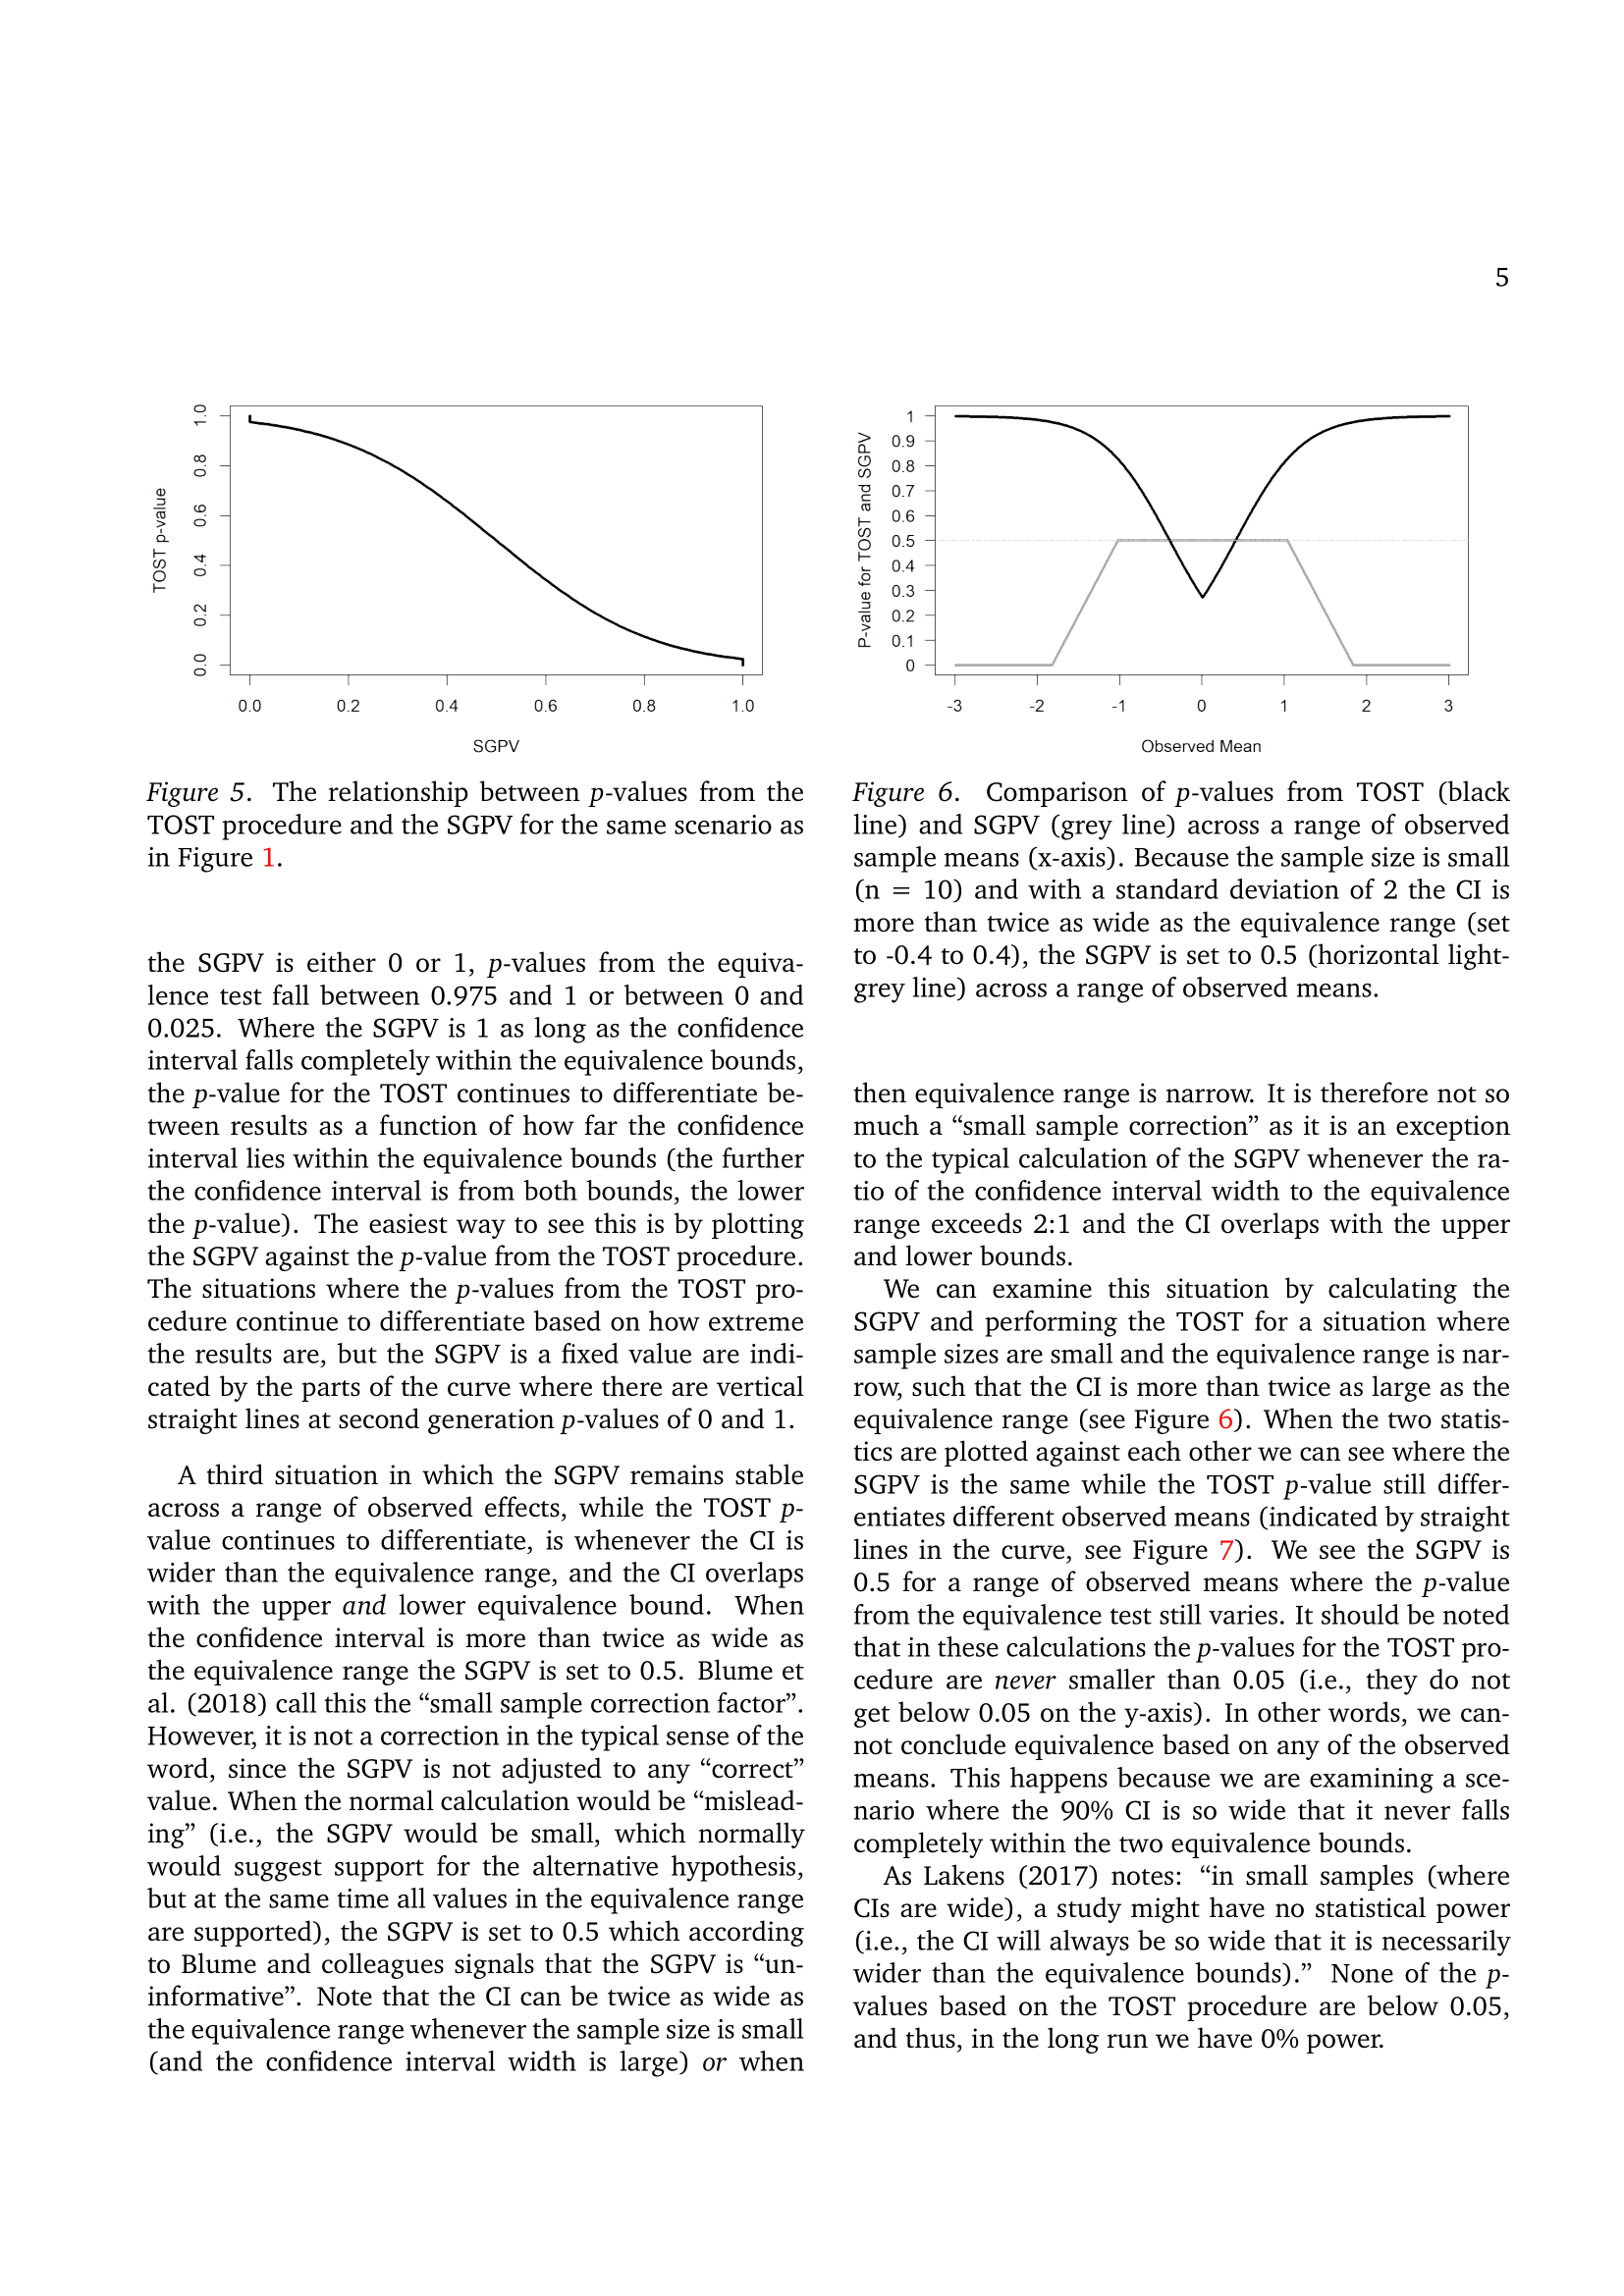
\includegraphics{C:/Users/Admin/Documents/Github projects/thesis/Chapitre 5/Chapitre 5-5} \end{center}

\begin{center}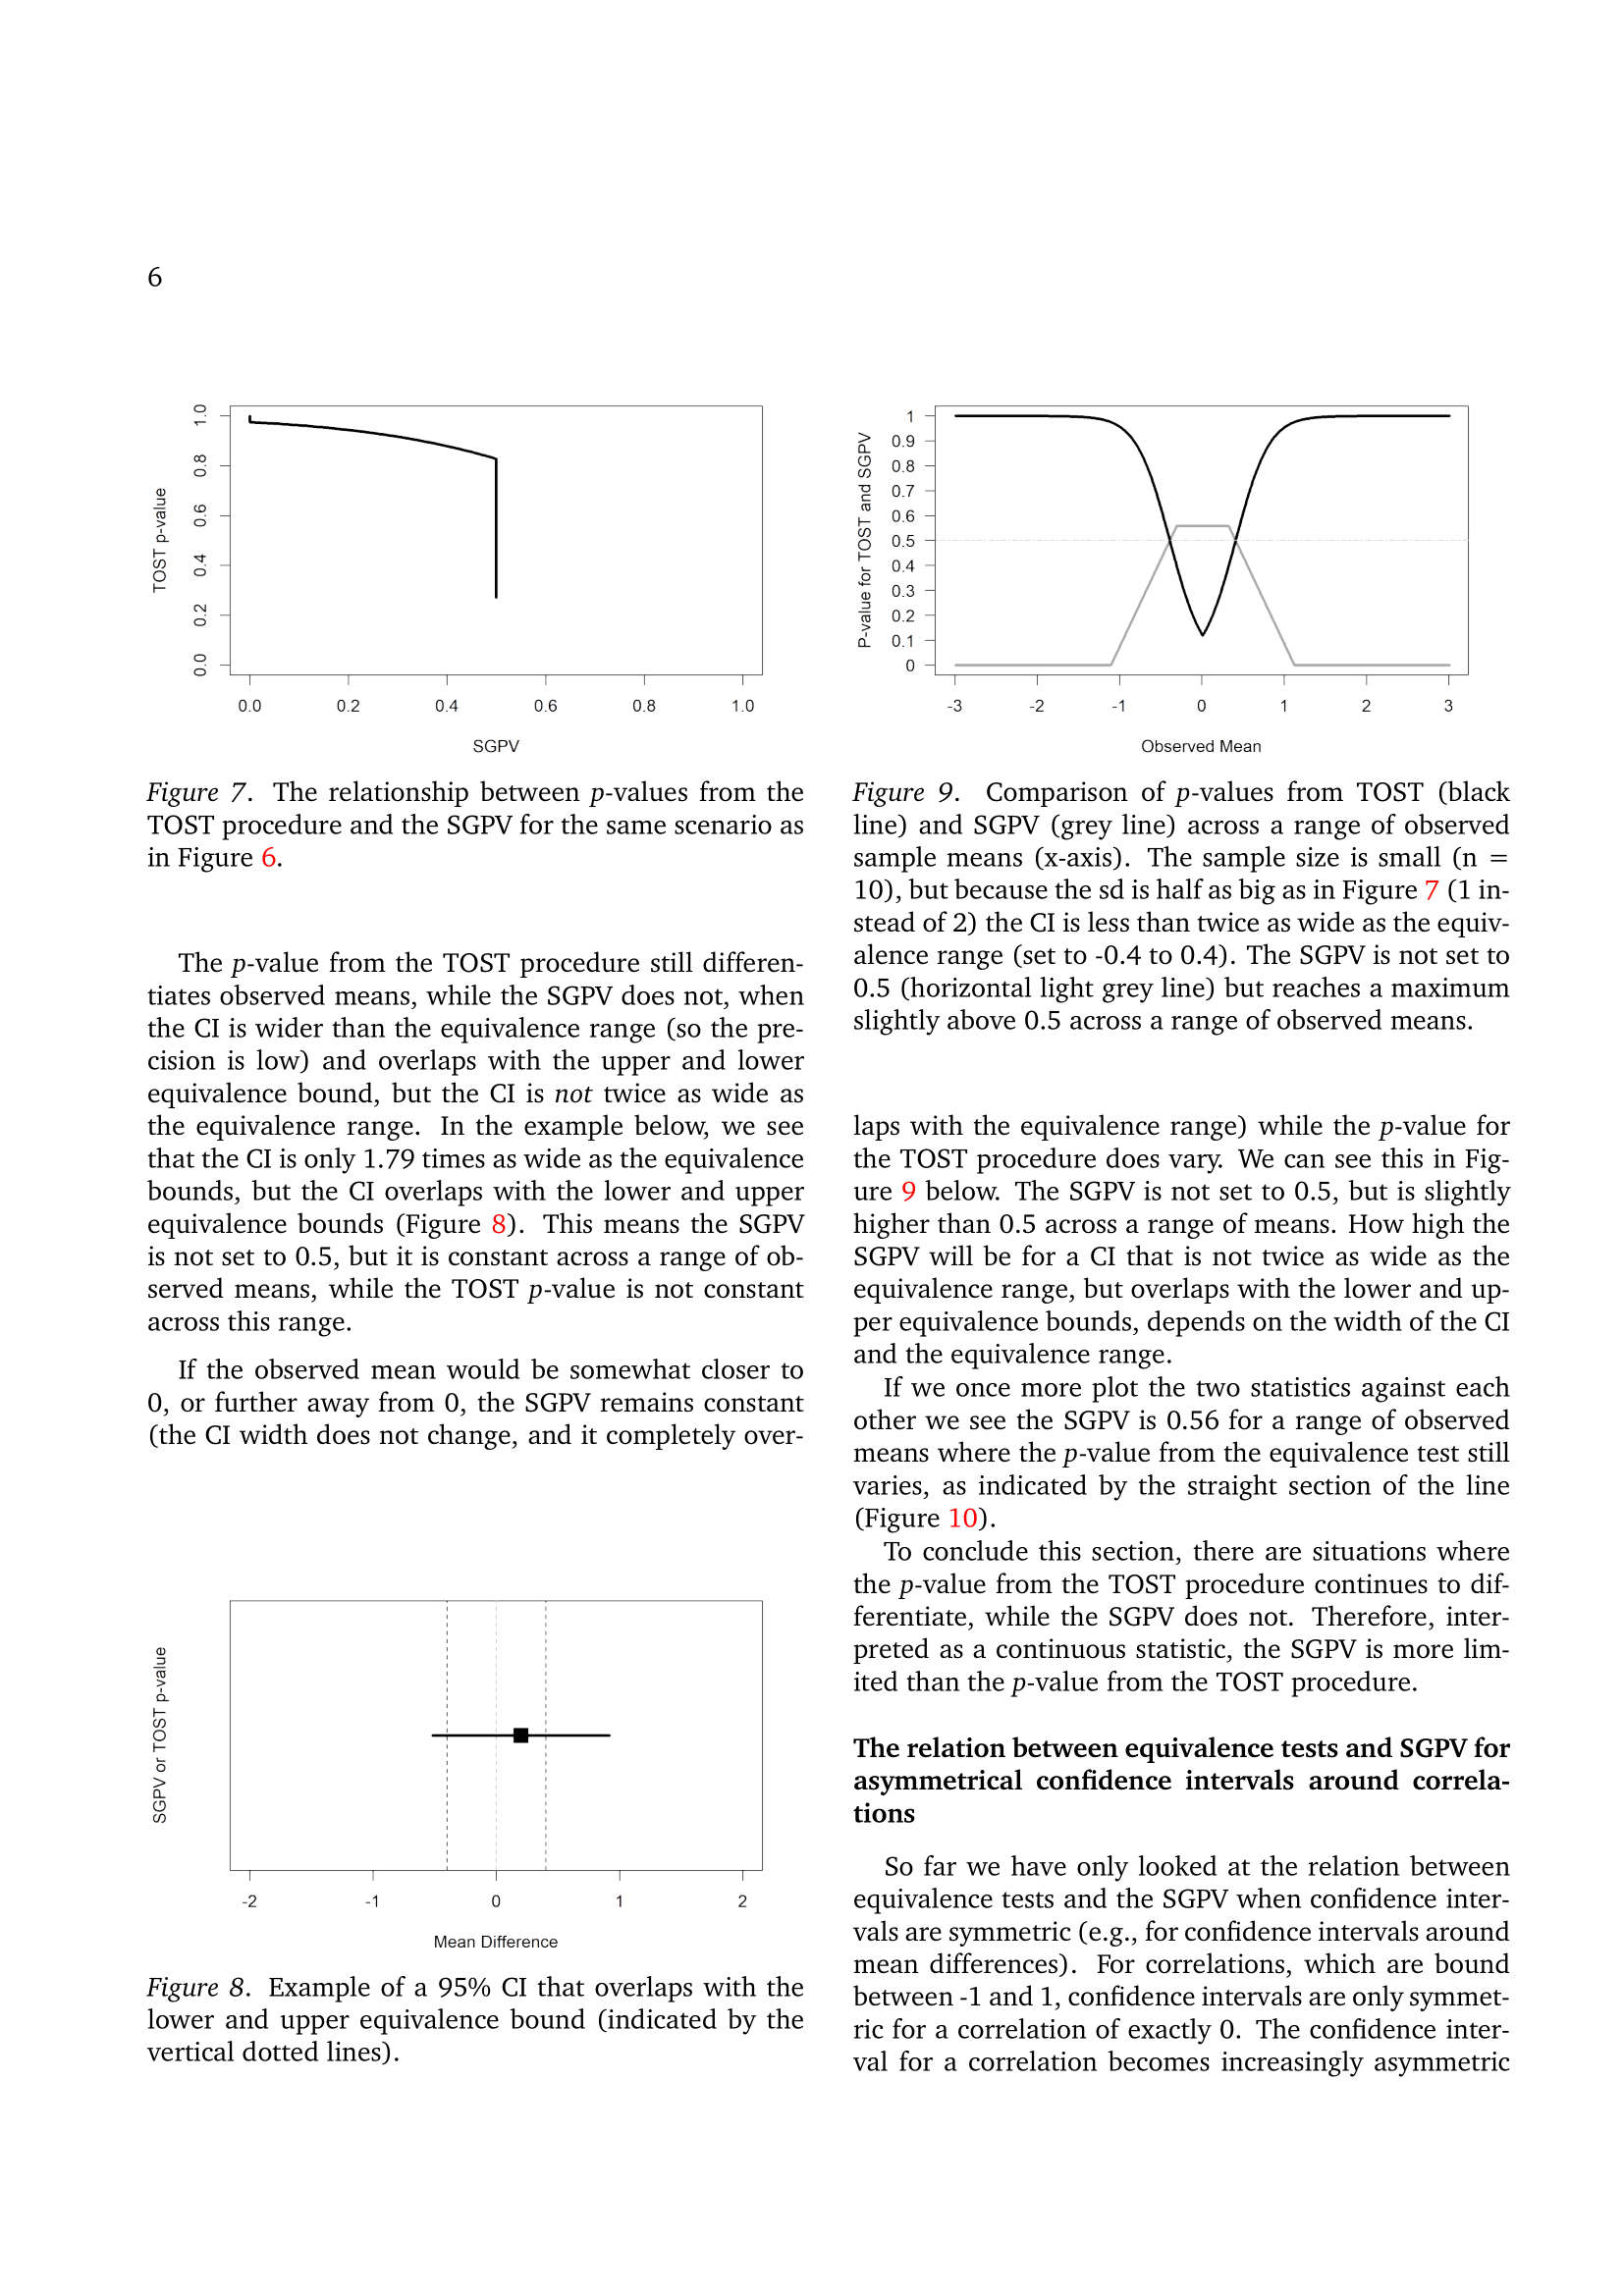
\includegraphics{C:/Users/Admin/Documents/Github projects/thesis/Chapitre 5/Chapitre 5-6} \end{center}

\begin{center}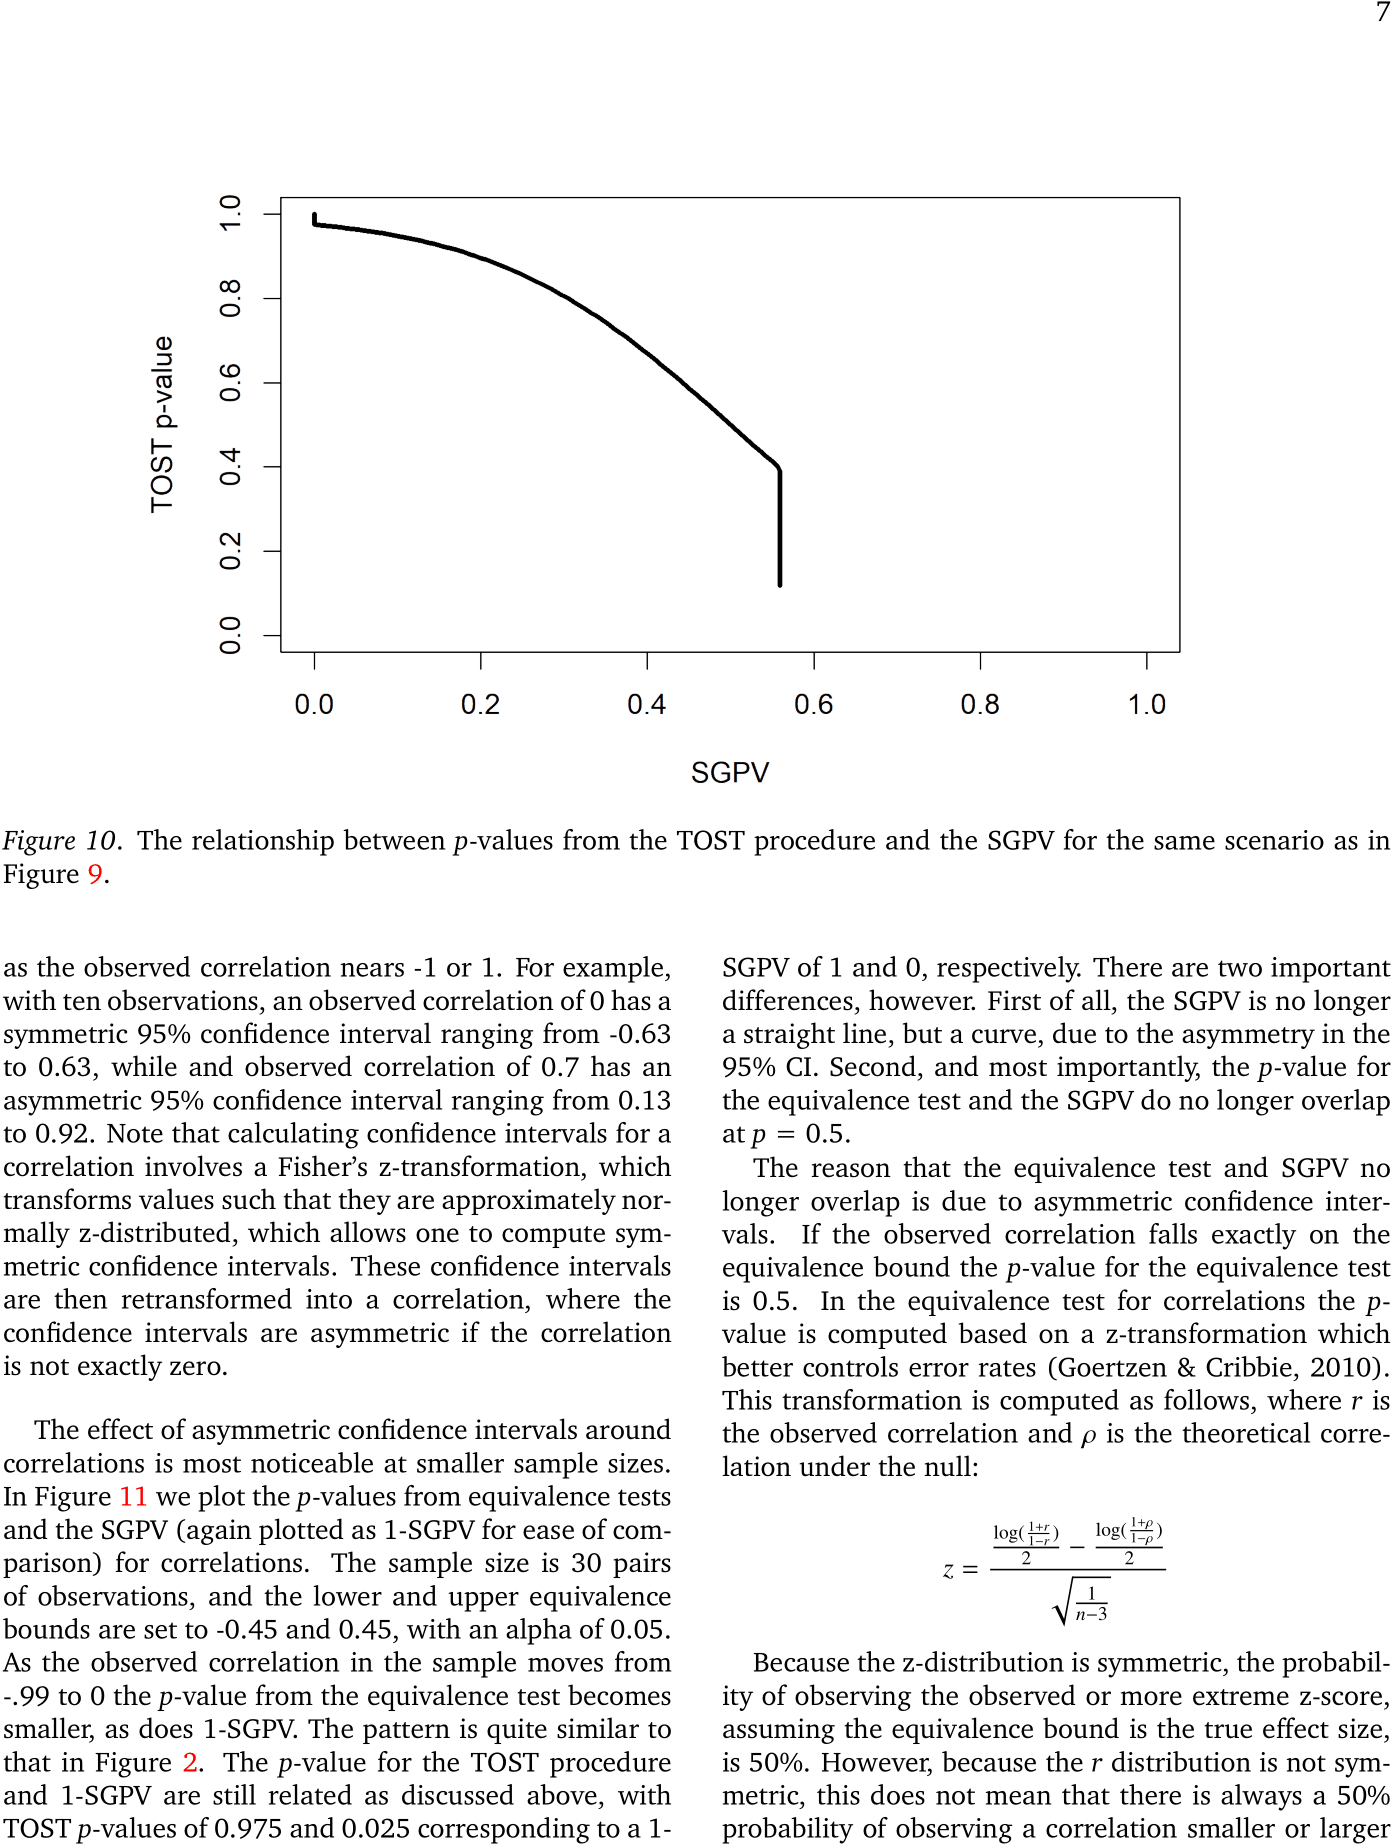
\includegraphics{C:/Users/Admin/Documents/Github projects/thesis/Chapitre 5/Chapitre 5-7} \end{center}

\begin{center}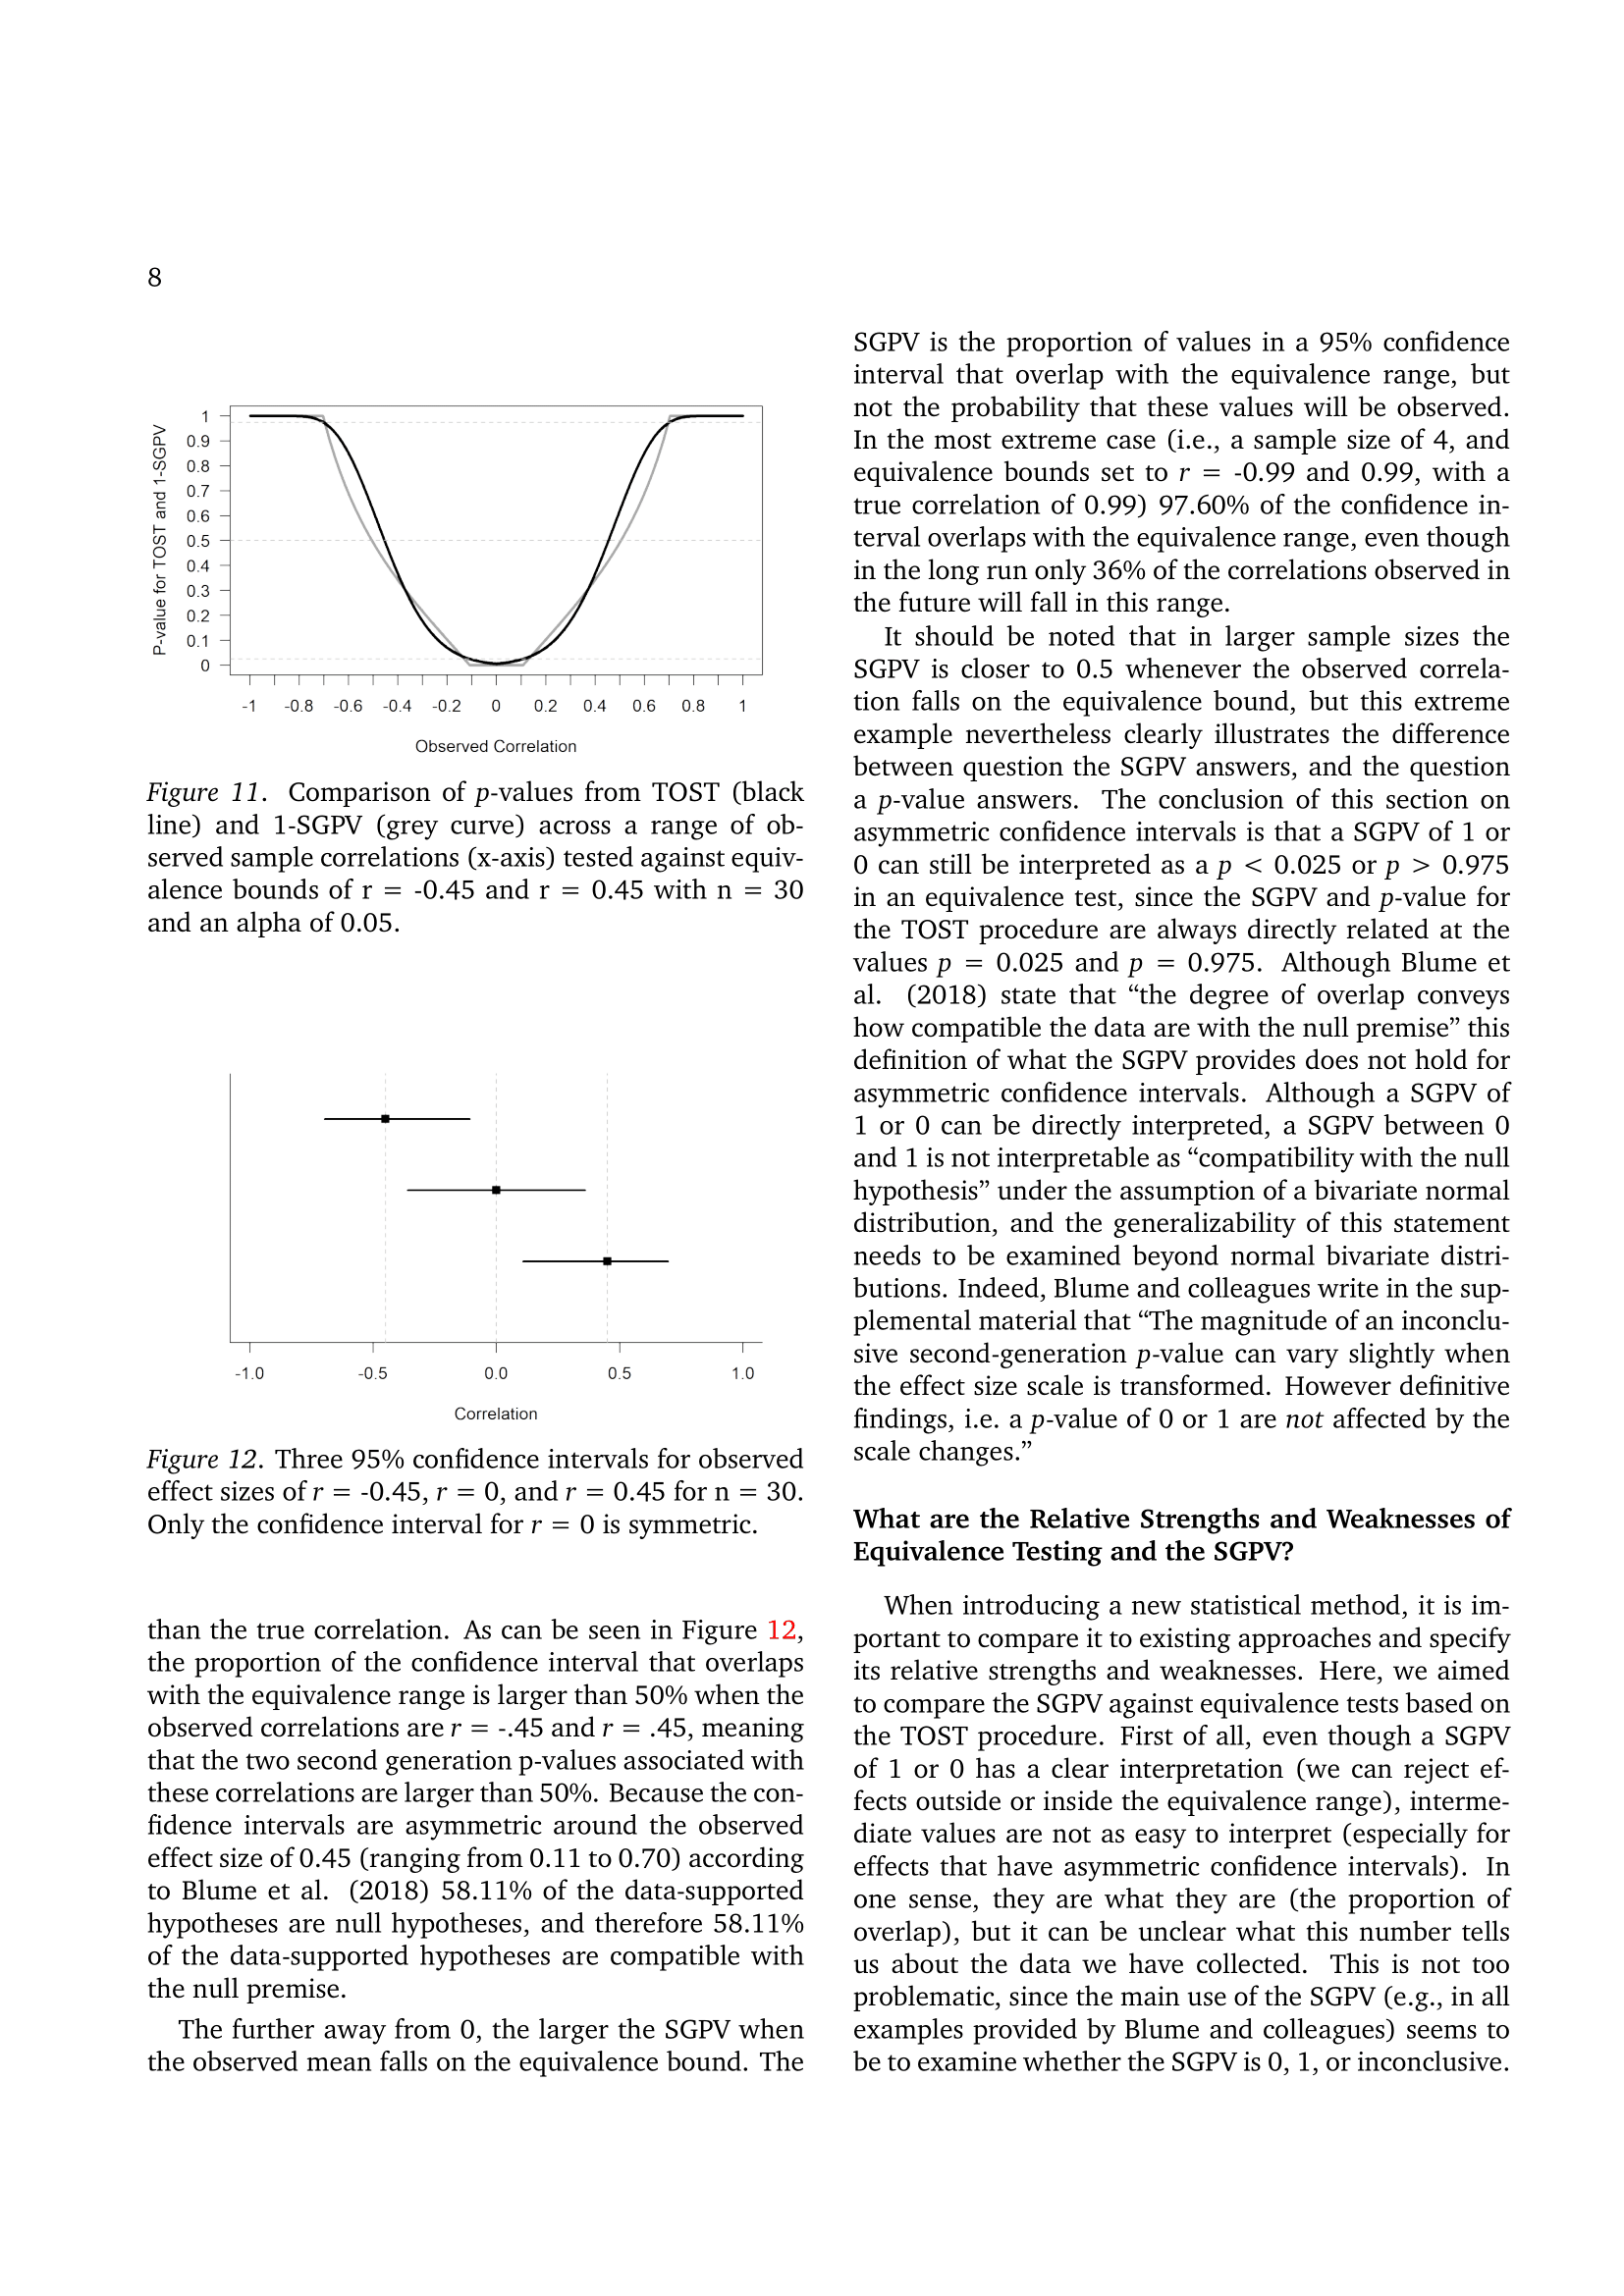
\includegraphics{C:/Users/Admin/Documents/Github projects/thesis/Chapitre 5/Chapitre 5-8} \end{center}

\begin{center}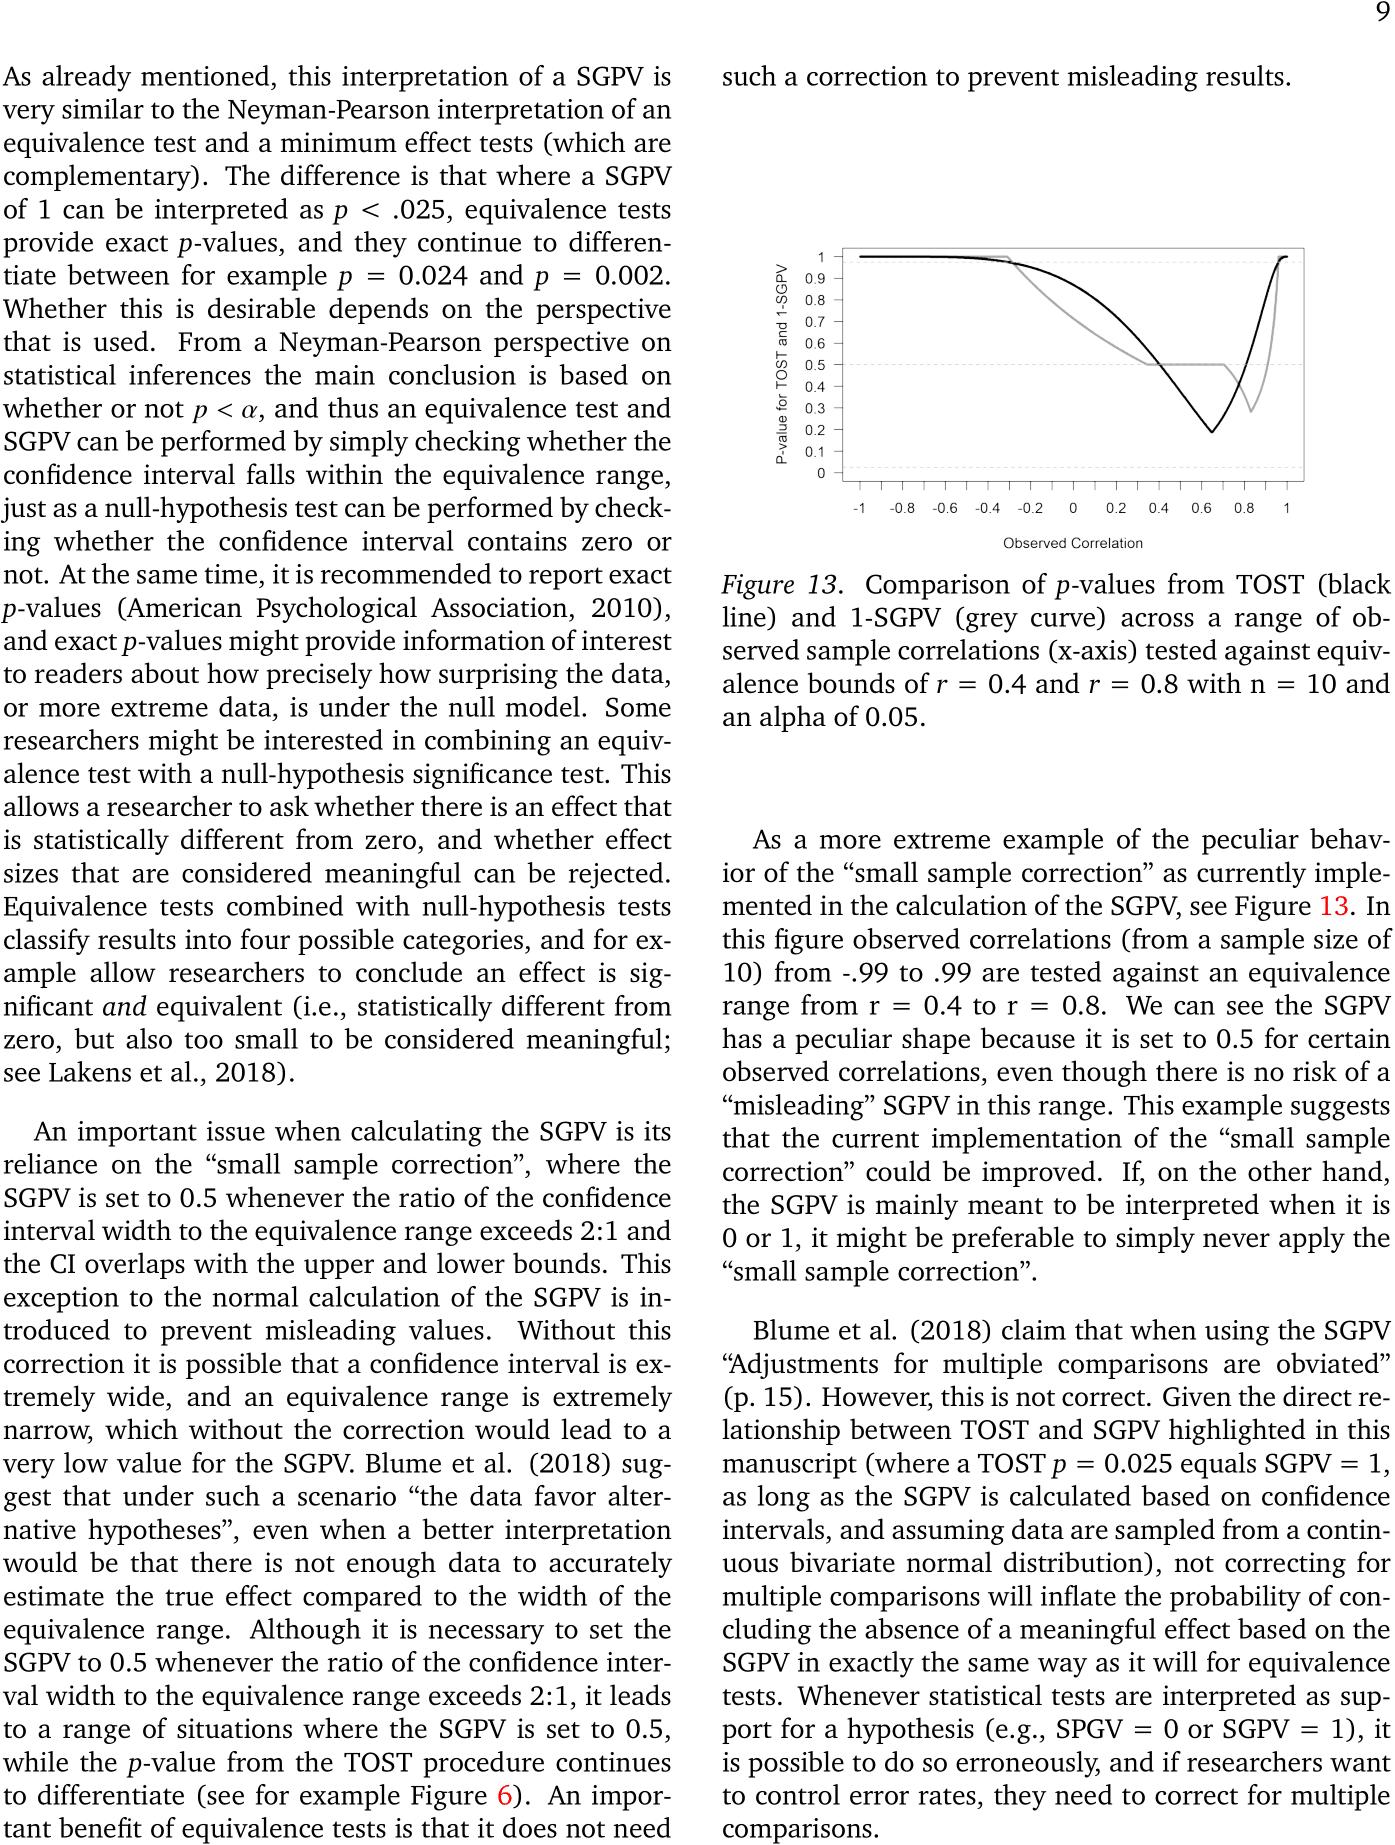
\includegraphics{C:/Users/Admin/Documents/Github projects/thesis/Chapitre 5/Chapitre 5-9} \end{center}

\begin{center}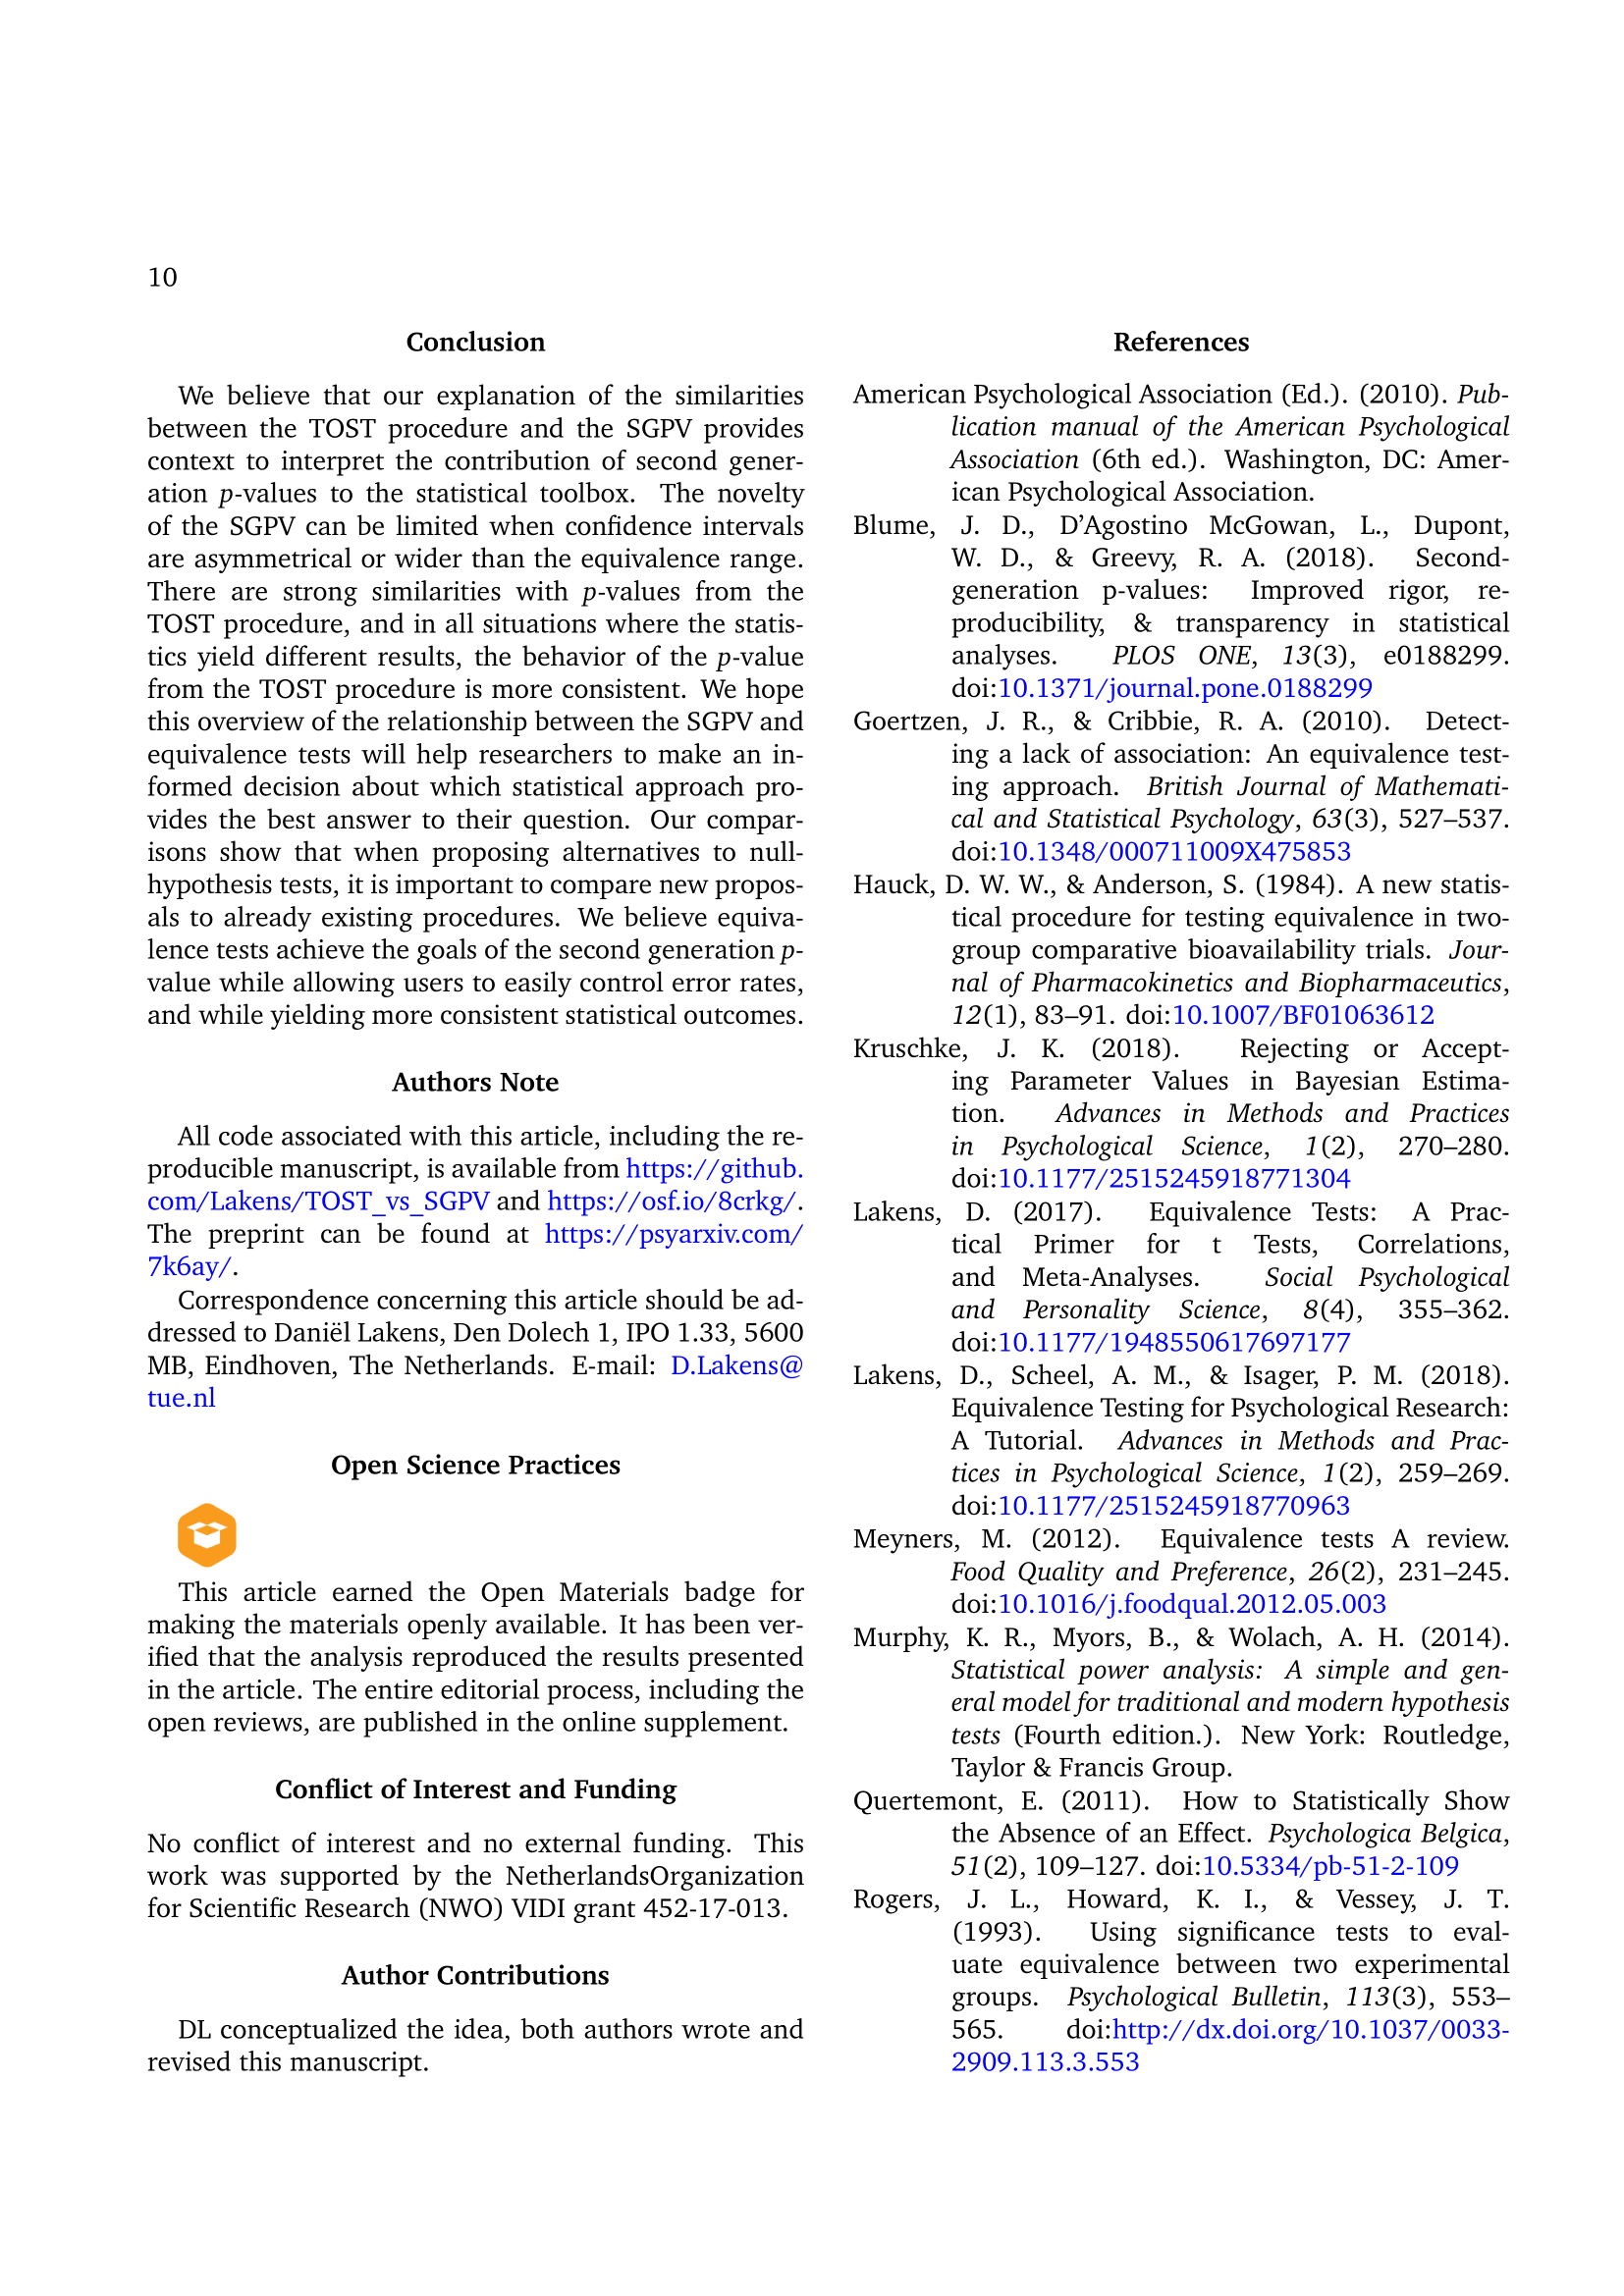
\includegraphics{C:/Users/Admin/Documents/Github projects/thesis/Chapitre 5/Chapitre 5-10} \end{center}

\begin{center}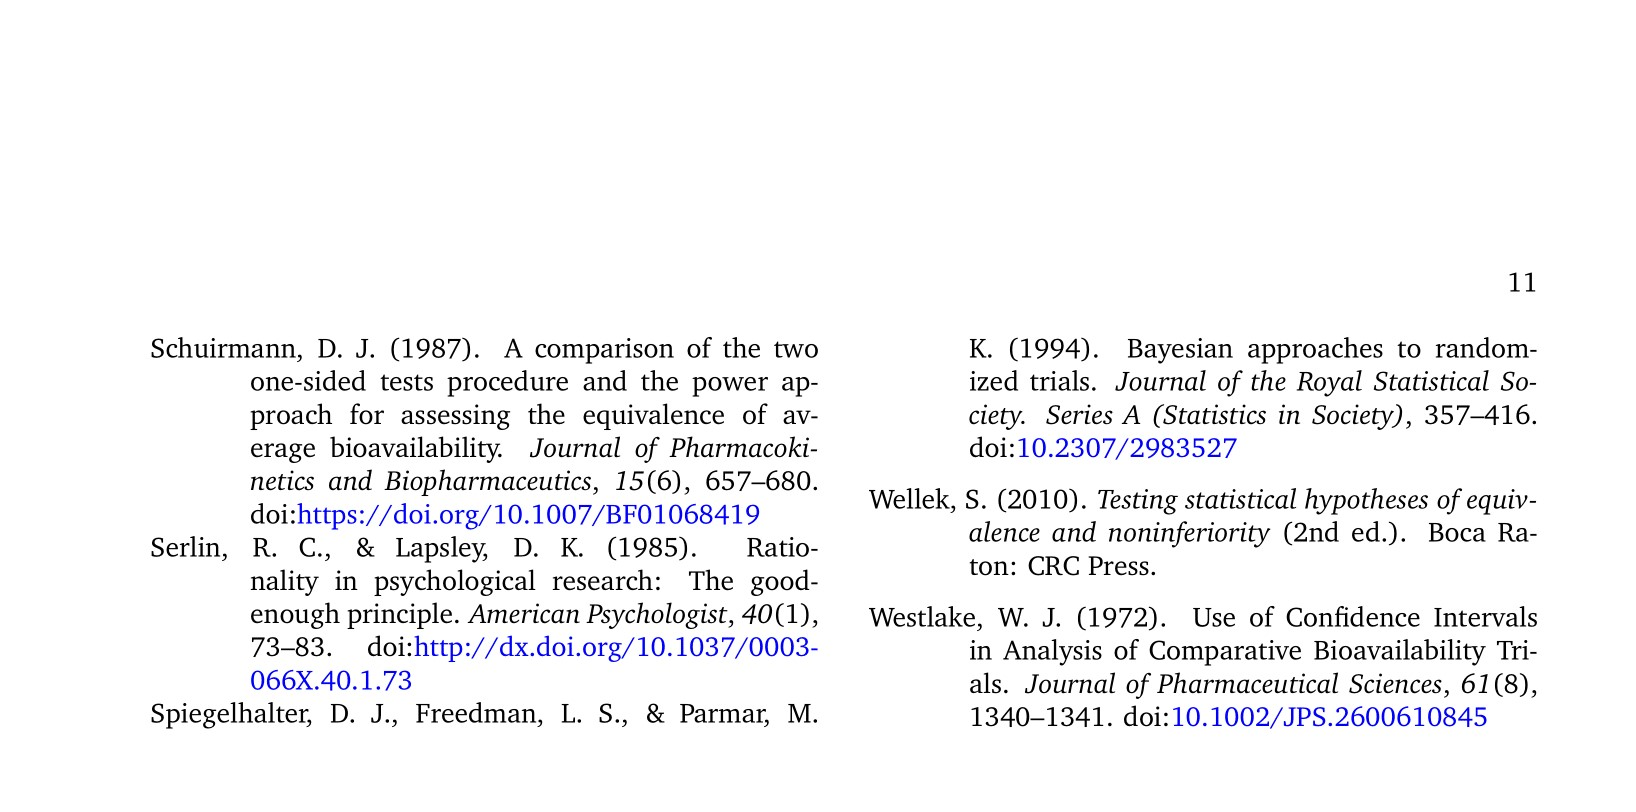
\includegraphics{C:/Users/Admin/Documents/Github projects/thesis/Chapitre 5/Chapitre 5-11} \end{center}


\end{document}
